\documentclass[10pt]{article}
\usepackage[utf8]{inputenc}
\usepackage[T1]{fontenc}
\usepackage{amsmath}
\usepackage{amsfonts}
\usepackage{amssymb}
\usepackage[version=4]{mhchem}
\usepackage{stmaryrd}
\usepackage{graphicx}
\usepackage[export]{adjustbox}
% babel包主要控制语言
\usepackage{babel}
\babelprovide[main, import, script=CJK, language=Chinese Simplified]{chinese}

% fontspec包主要控制字体
\usepackage{fontspec}
\setmainfont{AR PL SungtiL GB} % AR PL SungtiL GB是某个字体的名字,可替换成任何可以用的字体
\graphicspath{ {./images/} }
\usepackage{hyperref}
\hypersetup{colorlinks=true, linkcolor=blue, filecolor=magenta, urlcolor=cyan,}
\urlstyle{same}

\title{StreamPIM:在赛道内存中的流矩阵计算 }


\author{Yuda An $^{* 1}$, Yunxiao Tang ${ }^{* 1}$, Shushu Yi $^{1}$, Li Peng ${ }^{1}$, Xiurui Pan ${ }^{1}$\\
Guangyu Sun ${ }^{1,3}$, Zhaochu Luo ${ }^{1}$, Qiao Li $^{2}$, Jie Zhang ${ }^{1}$\\
Computer Hardware and System Evolution Laboratory,\\
Peking University ${ }^{1}$, Xiamen University ${ }^{2}$,\\
Beijing Advanced Innovation Center for Integrated Circuits 3\\
https://www.chaselab.wiki}
\date{}


\begin{document}
\maketitle


\begin{abstract}
赛道内存 (RM) Racetrack memory (RM)技术已经成为解决内存墙问题的有前途的解决方案,因为它们增加了内存密度,降低了能耗,并且能够构建内存中处理(PIM)架构。 RM可以将算术逻辑单元放置在其内存阵列中或其附近,以处理由主机卸载的任务。虽然已经有许多关于RM处理的研究,但不幸的是,这些解决方案都受到内存核心和计算单元松散耦合所带来的数据传输开销的影响。为了解决这个问题,我们提出了一种新的RM中处理架构StreamPIM,它将内存核心和计算单元紧密耦合在一起。具体来说,StreamPIM直接从畴壁纳米线构建矩阵处理器,而不使用基于cmos的计算单元。设计了一种基于畴壁纳米线的总线,消除了电磁转换。StreamPIM通过利用RM内部并行性进一步优化性能。我们的评估结果表明,与传统计算平台相比,StreamPIM实现了39.1倍的性能提升,节省了58.4倍的能耗
\end{abstract}

\section*{I. Introduction}
在过去的十年中,新兴的大规模应用,如机器学习,科学计算和图形分析 [23], [28], [42], [50],,由于它们对广泛的研究和工业领域的影响,受到了相当大的关注 [3], [60], [67]。 
与传统应用程序相比,这些应用程序既数据密集又计算密集。这是因为这些应用通常需要大规模的矩阵计算,这些计算需要大量的内存来存储矩阵的所有元素,并且需要大量的计算能力。例如,一种流行的机器学习模型, GPT-3 [11],  1750 亿个参数,需要高达 $800 \mathrm{~GB}$ 的内存和一个 1024 节点的集群进行 34 天的计算 [51]。最先进的语言模型, GPT-4 [55], 据报道拥有更多的参数,消耗更多的内存和计算能力。

大规模应用程序的持续发展刺激了对更大内存容量和更高计算能力的需求增长  [33], [74]。 不幸的是,现有的计算系统由于两个原因没有跟上大规模应用程序的快速发展。

\begin{center}
\begin{tabular}{|c|c|c|c|c|c|}
\hline
Memory & Access & Density & Energy & Reliability & PIM integration \\
\hline
DRAM & fast & low & high & high & CMOS [64] \\
\hline
PCRAM & slow & high & low & low & CMOS [43] \\
\hline
ReRAM & slow & high & low & low & in-cell [14] \\
\hline
MRAM & fast & low & low & high & \begin{tabular}{c}
CMOS [31] \\
in-cell [19] \\
\end{tabular} \\
\hline
RM & fast & high & low & high & \begin{tabular}{c}
CMOS [53] \\
skyrmion [45] \\
\end{tabular} \\
\hline
\end{tabular}
\end{center}

表 I: 不同内存技术的比较.


首先,传统的存储系统是基于DRAM构建的,面临着多个技术缩小规模的挑战。具体来说,DRAM存在保持时间违规、感知边际不足和低可靠性等限制[30], [36], [37], [48]。其次,被广泛采用的冯·诺伊曼架构[7], 遭受着数据移动带来的巨大开销。例如,研究 [13], [24] 表明,将数据从存储器移动到处理器的能量消耗比在处理器中进行数据处理要高出$3 \times \sim 11 \times$倍。

非易失性内存 (NVM) [18], [58] 已成为取代DRAM作为主存储器的一个有前途的候选方案。NVM可以提供比DRAM更高的内存密度。它还支持内存中处理(PIM)技术[14], [31], [43] 以实现内存内的并行矩阵计算,从而可以消除数据移动的开销。表I  总结了不同NVM解决方案的主要特性。虽然 阻抗性随机访问存储器 (ReRAM) [40], [79] 在内存密度和能耗方面优于DRAM,但由于其容易出错的固有特性,ReRAM容易受到可靠性问题的影响 [39]。 相变随机存取存储器(PCRAM) [12], [62]可以解决可靠性问题,但其访问延迟比DRAM要长得多。自旋转移磁阻存取存储器(STTMRAM) [17], [25] 的延迟比DRAM短。不幸的是,STT-MRAM的内存密度较低,使得它难以直接取代DRAM。磁畴壁内存 (DWM) [26], [57], 也称为赛道存储器(RM),在性能、能耗、密度和可靠性要求之间实现了良好的平衡(参见表 I)。

多项研究已经探索了在赛道存储器RM内处理矩阵计算的设计空间 [45], [53], [80]. SPIM [45] 提出在赛道存储器中集成多个基于skyrmion的计算单元,每个计算单元处理相邻存储核心中存储的数据。相比之下,DW-NN[80], 则采用基于CMOS的替代计算单元,这在器件制造上更加实用。 CORUSCANT [53], 是最先进的在赛道存储器内进行处理的工作,也采用基于CMOS的计算单元。它利用一种称为横向读取的机制 [63],以实现更低的计算延迟和更高的可靠性。然而,尽管PIM有诸多好处,以前工作中的计算单元需要反复从存储核心加载数据并将中间结果存回,这会产生数据转换的开销(例如,电磁转换)。考虑到赛道存储器的写入延迟和功耗相对较高 [82], 先前的方法受到了这种转换开销的影响。为了定量分析内存访问的密集性如何影响整体性能,我们通过检查CORUSCANT中各种类型的算术操作来对执行时间和能耗进行了详细的分析(详见图4)。在RM数组和计算单元之间传输数据分别占总执行时间和能耗的 $69 \%$ and $70 \%$ 。


为了解决上述挑战,我们提出了一种新的用于赛道存储器内进行处理的架构,称为StreamPIM,它利用RM独特的移位操作来消除计算单元和内存阵列之间传统读写操作所带来的数据转换开销。具体地,StreamPIM直接从域壁纳米线构建矩阵处理器 ( $R M$ 处理器) 该处理器通过移位操作进行计算,而无需使用基于CMOS的计算单元。与传统的设计用于标量操作的计算单元不同,RM处理器被很好地定制用于复杂的矩阵计算,消除了不必要的中间结果。为了提高在RM内的数据迁移效率,StreamPIM提出了基于域壁纳米线的总线( $R M$ 总线). 这种新总线通过移位操作直接传输数据,避免了电磁转换。StreamPIM通过利用RM内部的并行性,并以流水线方式传输数据和进行数据处理,进一步加速了矩阵处理。对于矩阵计算基准和端到端应用程序,我们的评估表明,与传统计算系统相比,StreamPIM分别实现了平均性能提高 $39.1 \times$ and $29.63 \times$ 。

我们的贡献点总结如下:

\begin{itemize}
  \item 针对流处理的新RM内处理架构:我们提出了一种新的RM内处理架构,其中计算单元和赛道存储器内部总线均完全由域壁纳米线构建。通过这样做,StreamPIM通过简单的RM移位操作执行计算和数据传输,而无需电磁转换,从而消除了RM的访问开销。此外,由于StreamPIM只使用移位操作,数据可以以流式方式移动和处理,提高了系统的吞吐量。
  
  \item 定制的矩阵计算RM处理器设计:传统PIM中的计算单元仅支持少数几种简单的算术操作。在大规模矩阵计算过程中,它们会产生大量中间结果,导致频繁的RM访问。相反,我们设计了一个定制的RM处理器,以流式方式执行整个矩阵计算。我们的RM处理器利用扇出机制[71]和域壁二极管[47]执行各种矢量操作,如加法、标量-矢量乘法和点积。

  \item 基于域壁纳米线的总线设计:为了减轻电磁转换带来的数据传输开销,我们的StreamPIM将基于电的总线替换为基于域壁纳米线的新型总线。因此,数据传输通过域壁纳米线上的移位操作来执行。然而,由于域壁纳米线的固有特性,这种新设计存在三个主要限制:(1)传输长度的不确定性;(2)由于高延迟而导致的低吞吐量;(3)由于距离较长而导致的移位故障问题。为了克服这些挑战,我们提出将新总线分成相同长度的段。在每个时钟周期,总线中的数据被移动一个段的长度,确保传输长度保持恒定。

  \item 用于并行矩阵处理的架构设计:我们引入了一个跨层设计,以更好地利用RM的内部并行性。具体来说,RM处理器集成在每个存储器数组中,将硬件并行性带到子阵列级别。矩阵表示和放置被精心设计以从软件方面利用硬件并行性。最后,在矩阵操作中,基本的数据复制和准备与显式计算分离,解决了RM读/写和移位操作之间的阻塞问题,以便进行并行性探索。

\end{itemize}

\section*{II. BACKGROUND}
\section*{A.  $R M$的总体架构}
内存核心。域壁内存(DWM),或称为赛道存储器(RM),是一种新型的基于自旋电子学的非易失性存储技术[56], [72]。在本文中,我们将DWM和RM互换使用。RM主要由多个域壁(铁磁性)纳米线组成,在先前的工作中也称为赛道。图1显示了域壁纳米线的核心结构,其中包含多个由域壁分隔的域。每个域存储一个比特数据,其值由磁化方向确定。因此,域壁纳米线能够存储多个位。域壁纳米线包含一个或多个访问端口,用于执行读写操作。访问端口是一个具有固定参考磁化方向的铁磁性组件。一个域和一个访问端口一起形成了磁隧道结构(MTJ)。要从域中读取数据,需要将读取电压应用到MTJ上。目标域和参考之间磁化方向的比较确定了MTJ的磁阻。读取操作利用此特性来感知位值。写入域是将高写入电流施加在MTJ上,这可以改变目标域的磁化方向。因此,RM的写入延迟和能量比RM的读取操作要高得多。

\begin{center}
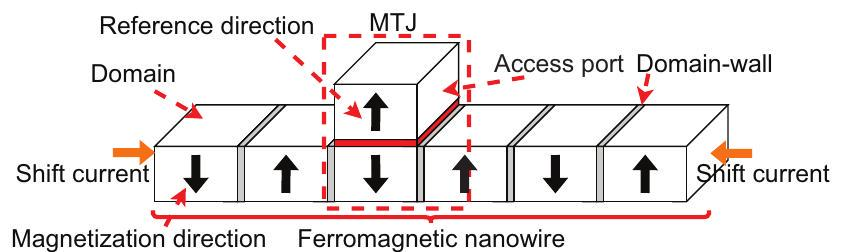
\includegraphics[max width=\textwidth]{2024_05_12_abeba8a85da5b5ec4c7bg-03(1)}
\end{center}

图1:域壁纳米线的核心结构。

\begin{center}
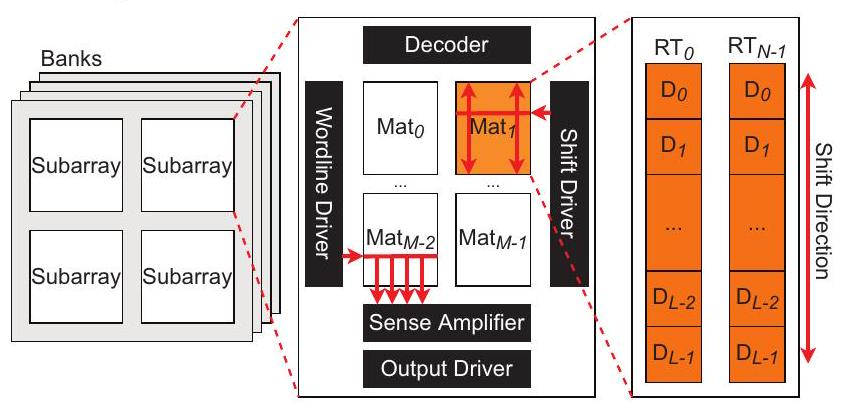
\includegraphics[max width=\textwidth]{2024_05_12_abeba8a85da5b5ec4c7bg-03(5)}
\end{center}

图2:赛道存储器的典型架构。

考虑到访问端口的成本,多个域被分组共享同一个访问端口。因此,RM需要一种操作,将特定域移动到与访问端口对齐的位置,然后进行读取或写入,这被称为移位操作。要执行移位操作,纳米线的两侧都连接有一个移位端口。通过移位端口向整个纳米线施加自旋极化电流来执行移位操作[26]。在施加电流期间,域和域壁将同步沿电流方向移动。具体而言,移位电流的持续时间和密度由移动数据的长度和移位距离决定。此外,为了避免移位时的数据丢失,在纳米线的两侧额外保留了一些域。保留域的数量取决于访问端口的数量,并且不会超过常规域的数量[82]。

内存组织。图2显示了一个典型的RM架构。类似于基于传统DRAM的内存,RM包括多个银行,每个银行包含几个子阵列。每个子阵列包括多个矩阵和外围电路,包括命令译码器、字线驱动器、感应放大器、输出驱动器和移位驱动器。每个矩阵是一组域壁纳米线。我们将纳米线和域分别表示为 $R T_{i}$ and $D_{j}$。需要注意的是,子阵列是为内存请求提供服务的基本单位。通过在银行和子阵列之间交错请求,所有银行中的所有子阵列都可以同时提供请求服务。

内存集成的挑战。目前,基于DRAM的尺寸缩放面临着多重挑战,包括单元漏电和感应边际等方面,这些限制了下一代DRAM器件的密度[15], [30], [36]。相比之下,通过采用相对较小的单元面积,并将多个位紧密集成到一个纳米线中,RM可以实现存储级密度,有望解决密度问题[26], [27], [68], [69]。然而,RM不能缓解由处理器和内存之间的数据迁移引起的开销。图3显示了基于CPU和基于GPU的计算系统的执行时间分解。

\begin{center}
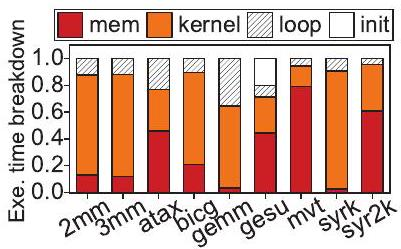
\includegraphics[max width=\textwidth]{2024_05_12_abeba8a85da5b5ec4c7bg-03(3)}
\end{center}

(a)CPU上的执行时间分解。


\begin{center}
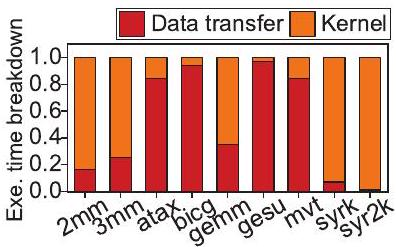
\includegraphics[max width=\textwidth]{2024_05_12_abeba8a85da5b5ec4c7bg-03(4)}
\end{center}

(b)GPU上的执行时间分解。\\
图3:CPU/GPU平台上的执行时间分解。


\begin{center}
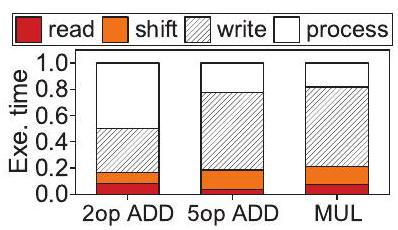
\includegraphics[max width=\textwidth]{2024_05_12_abeba8a85da5b5ec4c7bg-03(2)}
\end{center}

(a)执行时间分解。

\begin{center}
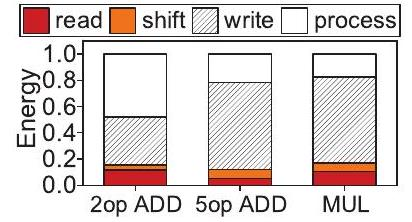
\includegraphics[max width=\textwidth]{2024_05_12_abeba8a85da5b5ec4c7bg-03}
\end{center}

(b)能量成本分解。

图4:CORUSCANT中支持的操作的执行时间和能量成本分解。

这些统计数据来自真实的平台,分别包含一个16核处理器[1]和一个GPU[2]。在基于CPU的计算系统中,小工作负载(即atax、bicg、gesu和mvt)的内存访问延迟(参见图3a中的mem)平均占总执行时间的47.6%。当在基于GPU的计算系统中执行相同的工作负载时,这一比例增加到90.0%(参见图3b中的数据传输)。这是因为GPU设备需要在主内存和其本地内存之间复制数据,从而增加了数据迁移的开销。

\section*{B. Racetrack Memory中的处理}
为了解决上述挑战,先前的研究[45],[53],[77],[80]通过在内存阵列内或附近放置定制的计算单元,构建了基于RM的处理内存(PIM)。由于数据在内存内直接处理,因此PIM方法避免了CPU/GPU与内存之间不必要的数据传输。然而,先前的方法仍然受到在内存核心和PIM计算单元之间进行数据转换带来的开销的影响。

具体而言,DW-NN [80]提议将基于CMOS的算术单元放置在RM阵列附近。数据从RM阵列中读取,然后由算术单元进行处理。最终的中间结果最终被写回RM阵列以进行后续操作。容纳这些中间结果大大增加了RM写操作的数量,从而加剧了RM阵列和算术单元之间的电磁转换开销。这是因为RM具有较长的写入延迟和较高的写入能量消耗。DW-AES [77]将AES加密的部分实现为RM的移位操作,从而减轻了数据转换开销。然而,这种方法高度依赖于特定算法,不能用于在一般的矩阵加法和乘法中减少此类开销。

最先进的工作CORUSCANT [53]利用了RM称为横向读取的独特特性,以减轻RM读取开销。
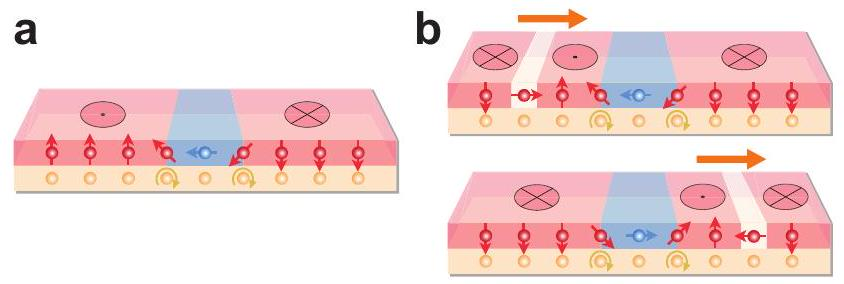
\includegraphics[max width=\textwidth, center]{2024_05_12_abeba8a85da5b5ec4c7bg-04(1)}
 
图5:领域壁纳米线逻辑机制


更准确地说,横向读操作同时感知一组连续的领域中的数据,而不是逐个访问每个领域。为了进一步减少操作延迟,CORUSCANT实现了另一个称为横向写的机制,它同时执行位移和写操作。尽管CORUSCANT由于新机制而具有比DW-NN更低的延迟和更高的可靠性,但由于必须从/向RM阵列提取/存储每个算术计算的中间结果,仍然会遭受电磁转换开销。为了弄清楚数据转换开销的影响,我们通过在CORUSCANT中执行三个常见操作来进行实验。具体来说,我们考虑了CORUSCANT中采用的特定操作过程,采用了现有的RM延迟和能耗模型的统计数据来进行模拟。图4a和4b分别显示了执行时间和能耗的细分情况。RM写操作占总执行时间的51.0%,而算术单元用于计算的执行时间仅为30.1%。同样,算术单元仅消耗总能耗的29.1%(参见图4b)。相比之下,RM写操作成为主要的能耗消耗者。总之,现有的PIM解决方案受到计算单元和存储阵列之间数据转换开销的影响。如何消除数据转换成为提高PIM性能和能效的关键。


\section*{III. 体系结构设计}
\section*{A. 关键观察}
最近,Luo等人 [46] 发现了一种物理机制,允许直接在领域壁纳米线上实现布尔逻辑操作。作者们还成功地制作了一个研究样本来演示基于RM的逻辑门。图5描述了他们的方法。具体来说,通过耦合磁性金属和重金属,将领域壁纳米线与领域壁反转器集成在一起。反转器用于启用称为Dzyaloshinskii-Moriya Interaction (DMI)的特殊相互作用 [22]。在图5b中,领域、领域壁和领域壁反转器分别用红色、白色和蓝色阴影标示。当领域和领域壁受到电流驱动(见图5b中的橙色箭头),因此在反转器上移动时,由于DMI的作用,领域的逻辑将被反转。因此,反转器相当于一个非门,因为它反转了领域的逻辑值。此外,通过DMI,可以将两个输入、一个偏置和一个输出领域耦合在一起,进行更复杂的逻辑操作。

\begin{center}
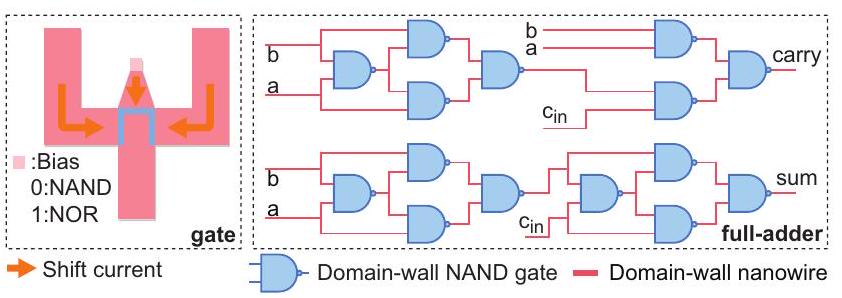
\includegraphics[max width=\textwidth]{2024_05_12_abeba8a85da5b5ec4c7bg-04}
\end{center}
图 6: 领域壁纳米线逻辑结构。

图6展示了领域壁NAND/NOR门的结构。根据给定的偏置,相应的逻辑操作可以是NAND或NOR。请注意,由于所有的布尔操作都可以通过NOT、NAND和NOR操作的组合来实现,因此可以基于领域壁纳米线构建一个具有完整功能的算术单元。我们在图6中描述了基于领域壁NAND门构建的一位全加器。

\section*{B. StreamPIM的内部架构}

上述机制允许将算术单元与存储阵列紧密集成。受到这一关键观察的启发,我们设计了基于领域壁纳米线的处理器和总线,并将它们集成到RM设备中,从而显著降低了处理-in-RM架构中的数据转换开销。

图7展示了我们称为StreamPIM的设计的内部架构。为了提供常规的内存访问服务,我们采用了传统的RM架构,包括三个级别,包括Bank、Subarray和Mat。Bank是顶层组件,可以独立运行。所有的Bank都通过共享的内部总线连接在一起,该总线支持必要的Bank间数据传输。一个Bank包含多个Subarray和外围电路模块,包括全局行缓冲区和行解码器。每个Subarray可以通过本地字线和位线进行访问,以支持内存访问操作。为了利用多Bank PIM架构带来的并行性,我们在每个Bank中添加了一个Bank控制器,以在内部提供PIM操作服务。Bank控制器通过PIM控制线管理其Subarray。此外,我们采用了一个先前工作[38]中启发的本地行缓冲区设计,该设计与每个Subarray耦合。这种设计提高了不同Subarray之间的并行性,并允许一个Bank容纳更多的Subarray。每个Subarray由多个RM Mat、一个RM Processor和一组内部RM总线组成。而RM Mat是基本的存储阵列,RM Processor作为主要的计算单元执行PIM功能。RM总线连接了Mat和Processor以进行数据传输。所有这些组件都是由领域壁纳米线构建的,以最小化处理过程中的数据转换。







\section*{C. RM 处理器}
我们的RM处理器专为矩阵计算而设计,包括标量加法、标量乘法和向量点积。为了支持标量加法,我们基于图6中所示的1位全加器设计构建了一个RM串行进位全加器。以下描述了我们的RM处理器设计如何支持各种乘法操作。

\begin{center}
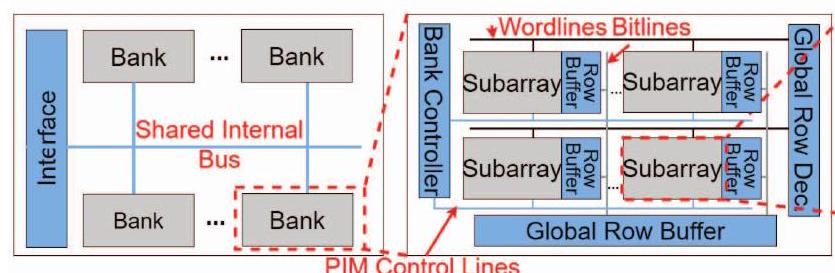
\includegraphics[max width=\textwidth]{2024_05_12_abeba8a85da5b5ec4c7bg-05(4)}
\end{center}

(a) Device

(b) Bank

\begin{center}
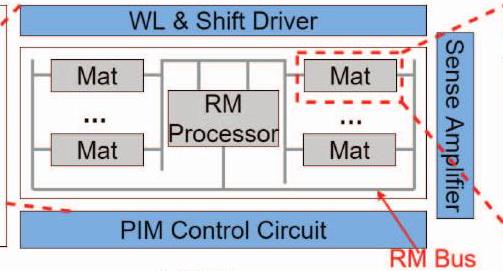
\includegraphics[max width=\textwidth]{2024_05_12_abeba8a85da5b5ec4c7bg-05(2)}
\end{center}

(c) Subarray

\begin{center}
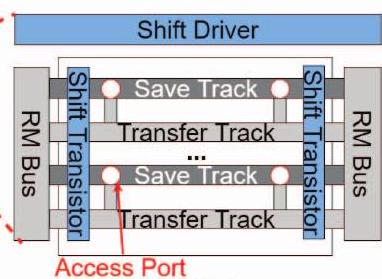
\includegraphics[max width=\textwidth]{2024_05_12_abeba8a85da5b5ec4c7bg-05(1)}
\end{center}

(d) Mat

图7:StreamPIM 设备架构。

\begin{center}
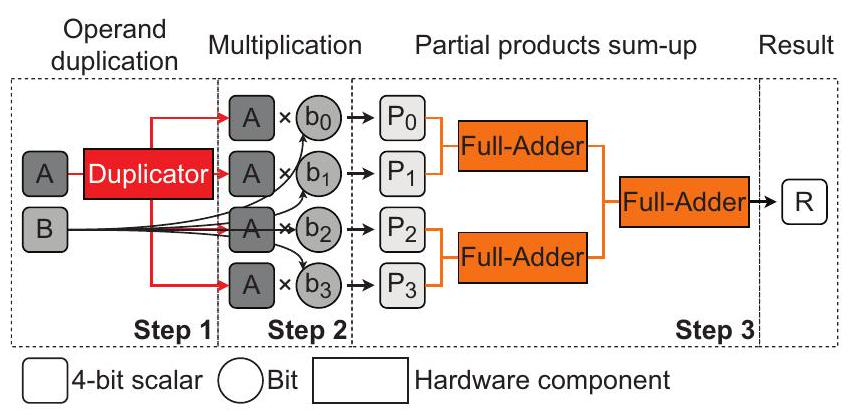
\includegraphics[max width=\textwidth]{2024_05_12_abeba8a85da5b5ec4c7bg-05(3)}
\end{center}


Fig. 8: 4位标量乘法示例。


标量乘法。图8展示了4位标量乘法的过程。需要注意的是,虽然我们的设计支持8位操作数,但由于空间限制,我们只展示了一个4位的示例。具体而言,标量乘法的硬件实现包括三个步骤:复制其中一个输入操作数(即复制 $A$ ),生成部分乘积(即 $A * b_{i}$ ),以及求和部分乘积。

在RM中,复制步骤并不简单,因为移位操作只能在磁域壁纳米线上移动数据,而不能复制数据。我们的解决方案受到了RM领域中两项材料级别创新的启发,即Fan-Out [46]、[71]和Domain-Wall Diode [47]。具体来说,Fan-Out方法设计了一个磁域壁纳米线的分叉结构。当在线的两侧施加电流时,输入的磁域在通过分叉点时会分裂成两个磁域。另一方面,类似于传统的二极管,磁域壁二极管允许磁域只在一侧可移动,当二极管被激活时。这个机制使得在纳米线上灵活控制数据移位方向成为可能。利用这两种机制,我们设计了一个称为复制器的硬件组件来执行数据复制。图9展示了复制器的结构以及复制数据的四个步骤。具体而言,复制器是由一个定制的磁域壁纳米线构建的,遵循Fan-Out机制。它在两个分支纳米线中的一个上放置了一个磁域壁二极管。复制过程如下:移位操作将数据传播到两个分支纳米线(步骤1)。当数据达到分支纳米线时,根据Fan-Out机制,磁域被复制(步骤2)。一份原始数据的副本经过启用磁域壁二极管以避免冲突后,被传送回到原始位置(步骤3)。数据返回到原始位置,准备好进行下一次复制(步骤4)。

\begin{center}
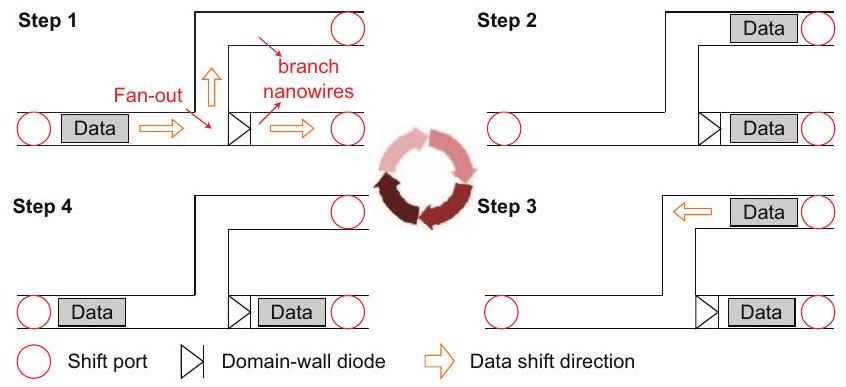
\includegraphics[max width=\textwidth]{2024_05_12_abeba8a85da5b5ec4c7bg-05}
\end{center}

图9:复制器结构和复制步骤。

 同时,另一个副本向前移动,执行后续操作。需要注意的是,一个$n$位标量乘法需要进行$n$次复制,这将导致$n$个周期的停顿。为了解决这一挑战,我们在处理器中采用多个复制器同时复制向量的不同部分,从而降低了复制的时间消耗。

在复制完成后,即可计算部分乘积及其总和(参见图8中的步骤2和3)。部分乘积可以通过二进制数据表示下的AND门简单生成。为了求和部分乘积,我们利用上述的RM全加器实现了多操作数加法器,通过加法树来实现(参见图6)。

向量点积。向量点积操作是将前述的标量乘积产生的结果求和(参见图8中的Result)。为此,我们提出了一种称为Circle Adder的设计,它由一个$n$位全加器、定制纳米线和磁域壁二极管组成。图10展示了其结构和将入射的标量乘积产品添加到累积结果的四个步骤。具体而言,全加器将入射的乘积值(d1)和累积结果(s1)作为两个操作数,生成一个新的累积结果(步骤1)。这个结果(s2)穿过磁域壁二极管(步骤2)。然后,s2通过由磁域壁二极管引导的环形纳米线返回到操作数位置(步骤3)。新的标量乘积结果($\mathrm{d} 2$)到达操作数位置,准备进行下一轮加法运算(步骤4)。加法过程将重复进行,直到所有标量乘积求和完成。然后,最终结果将被传输出去。需要注意的是,环形加法器也可以通过简单地将操作数在不发送结果的情况下通过全加器进行移位来执行标量加法操作。我们对环形加法器进行了多路复用,以执行加法和点积,从而简化了硬件设计。流水线处理器。图11展示了我们的RM处理器的总体结构,其中包括前述的复制器、乘法器、加法树和环形加法器。

\begin{center}
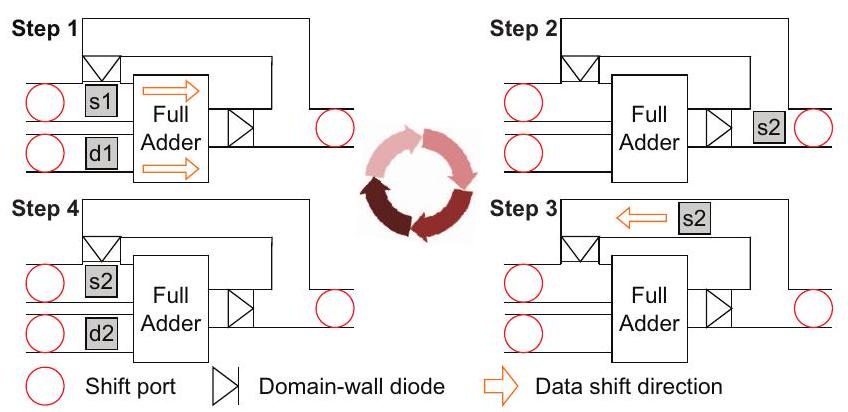
\includegraphics[max width=\textwidth]{2024_05_12_abeba8a85da5b5ec4c7bg-06(1)}
\end{center}

图10:环形加法器结构。

为了提高处理吞吐量并隐藏通过磁域逻辑门传输数据的非可忽略延迟,我们以流水线形式设计了RM处理器结构。具体地,我们将RM处理器分为四个阶段。在执行向量点积时,一系列标量操作数被获取到RM处理器中。当一个标量操作数被发送到复制器时,其他操作数被拆分为单独的位(阶段1)。复制器迭代地复制操作数,然后发送到乘法器。乘法器从这些副本生成部分乘积(阶段2)。接着,一个加法树将部分乘积相加以生成标量乘积的结果(阶段3)。一个环形加法器收集来自前一阶段的所有标量乘积结果并将它们相加(阶段4)。需要注意的是,我们的RM处理器还支持其他类型的矩阵操作。具体而言,标量乘法绕过环形加法器(阶段4),因为不需要将标量乘法结果相加。标量加法绕过复制器、乘法器和加法树(阶段1至3),而使用环形加法器作为简单的加法器。向量加法可以通过流水线化标量加法来执行。标量向量乘法通过反复复制其标量操作数并流水线化以下标量-标量乘法来执行。

\section*{D. RM 总线}

虽然 RM 阵列和 RM 处理器都是由领域壁纳米线构建的,但在它们之间传输数据需要进行电磁数据转换,这是由于传统的电气总线所致。受到 RM 移位操作是一种数据传输的启发,我们提出使用领域壁纳米线(RM 总线)构建 RM 内部总线。

优势。RM 总线带来两个主要优势。首先,通过使用领域壁纳米线进行数据传输,可以消除读/写操作。由于大规模的数据密集型应用可能会产生大量的读/写操作,精心设计的 RM 总线将有望优于传统的电气总线,后者经常遭受频繁的电磁转换的困扰。其次,领域壁纳米线允许复用,这在传统的电气总线中是不可行的。具体来说,领域壁纳米线由许多域组成,可以容纳来自不同 RM 阵列/处理器的数据。由于移位操作以流式方式移动所有域,因此可以在没有干扰的情况下同时传输不同的数据。

\begin{center}
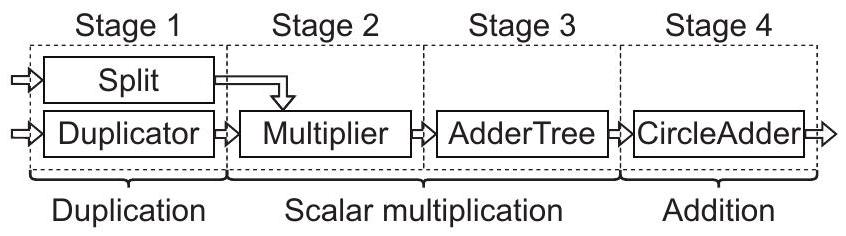
\includegraphics[max width=\textwidth]{2024_05_12_abeba8a85da5b5ec4c7bg-06}
\end{center}

Fig. 11: Pipelined RM processor.

\begin{center}
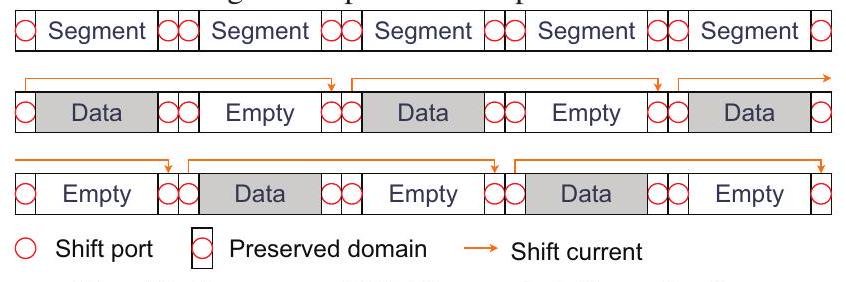
\includegraphics[max width=\textwidth]{2024_05_12_abeba8a85da5b5ec4c7bg-06(2)}
\end{center}

Fig. 12: RM 总线结构和移位机制。

相比之下,电气总线只能在任何给定周期传输一组数据。这些优势使得领域壁纳米线成为高性能数据传输的潜在选择。

挑战。在 RM 移位操作期间,电流脉冲被施加到领域壁纳米线中的特定方向。然后,数据通过领域壁纳米线传播。然而,这种移位机制引入了三个主要挑战。首先,电流脉冲的持续时间和密度需要由纳米线的长度决定。然而,由于数据的来源和目的地各不相同,很难确定不同传输的纳米线长度。电流持续时间和密度的不确定性使得控制 RM 总线变得具有挑战性。其次,RM 总线的数据传输延迟要比电气总线高得多,因为域只能以有限的速度在纳米线上传播。因此,单个数据的传输成本为多个周期,并且如果数据逐个传输,则吞吐量可能严重受限。第三,当纳米线的长度增加时,过度移位和不足移位故障会累积并变得严重,从而限制了传输距离。

我们的设计。为了解决上述挑战,我们定制了 RM 总线的结构,如图 12 所示。具体来说,StreamPIM 将领域壁纳米线中的几个连续的域分组为一个段。然后,将每个领域壁纳米线分成相同长度的多个段。在段的两侧,保留一个域用作移位端口,该端口在领域壁纳米线上施加电流。在传输数据时,一个段处于两种不同状态之一,即携带数据或为空。图 12 描述了这两种状态。段的关键见解是在每个周期中仅将数据移位一个段的长度,限制了移位长度。因此,可以避免移位电流持续时间和密度的不确定性。然而,为了避免数据丢失,传输过程中应将数据段移至空段。因此,在传输方向上,一组数据段总是在空段之后。此外,相邻数据段之间意外的错位速度也会导致数据丢失。这一特性要求通过单个移位电流移动一组相邻的数据段。因此,由于纳米线的长度随相邻段的数量而变化,移位电流的持续时间和密度仍然存在不确定性。

\begin{center}
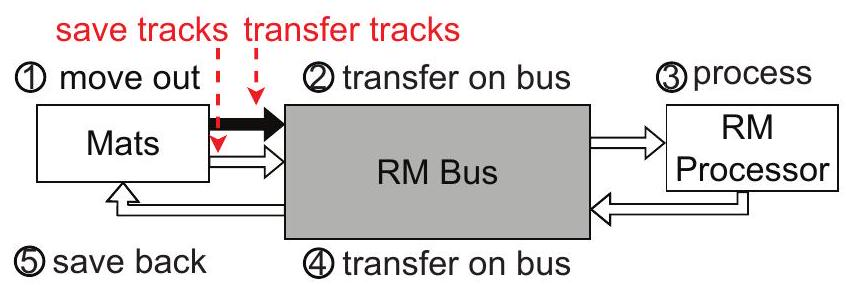
\includegraphics[max width=\textwidth]{2024_05_12_abeba8a85da5b5ec4c7bg-07}
\end{center}

Fig. 13: 单个子阵列中的 PIM 数据流。

为了完全消除这种不确定性,个别数据段被空段分隔开。因此,在传输方向上,一个数据段总是跟随一个空段(参见图 12)。因此,单个移位电流仅应用于一个数据段和相邻的空段。此外,通过同时对所有这些数据-空段对进行移位操作,可以以流水线方式并发传输来自不同来源的数据。与非流水线传输相比,这种流水线传输大大提高了 RM 总线的数据传输吞吐量,消除了相对较长的传输延迟的影响。此外,由于每个移位操作的移位距离仅限于一个段,因此可以缓解移位故障问题。总之,我们的设计通过巧妙地将 RM 总线分割为段来克服上述挑战,并且与传统总线相比,可以提供显著的性能改进,如我们的评估所示(参见图 19)。

\section*{E. 矩阵设计n}
我们提出了一种新的矩阵设计,以消除电磁转换并实现非破坏性读取操作,如图 7d 所示。矩阵本质上是一组域壁纳米线的阵列。请注意,矩阵中的域壁纳米线特别称为赛道。为了在没有电磁转换的情况下与 RM 总线通信,矩阵中的赛道被延伸并通过域壁纳米线连接到 RM 总线。因此,数据可以通过移位操作在矩阵和 RM 总线之间移动。但是,在移位操作之后,数据不会保留在原始的矩阵中。因此,从矩阵到 RM 总线的域的移位是一种破坏性读取操作。为了执行非破坏性读取,数据必须被复制到而不是移动到 RM 总线上。为此,几个矩阵中的赛道被划分为两种类型:保存赛道和传输赛道。保存赛道是用于容纳数据的基本单元。它们与访问端口连接,以执行常规的内存读/写操作。传输赛道用于非破坏性读取,只将数据发送到 RM 总线。传输赛道不与访问端口连接,而是通过扇出域壁纳米线连接到保存赛道(参见图 7d)。通过扇出机制,数据可以复制到传输赛道,而不会从保存赛道中擦除,复制品可以转移到 RM 总线上。如果需要非破坏性地读取一组数据,则它们将被传输到各矩阵的传输赛道上。








\begin{center}
\begin{tabular}{|c|c|}
\hline
Commands & Description \\
\hline
MUL src1,src2,des,size & Dot Product \\
\hline
SMUL src1,src2,des,size & Scalar-Vector Multiplication \\
\hline
ADD src1,src2,des,size & Vector Addition \\
\hline
TRAN src,des,size & Data Transfer \\
\hline
\end{tabular}
\end{center}

表II:向量处理指令(VPC)。

\section*{F. Subarray内部数据流程}
在Subarray内部处理PIM任务涉及到mats、RM总线和RM处理器。整个过程如图13所示。由于数据最初驻留在mats中,数据首先需要从mats转移到RM处理器。通过应用移位操作,数据从mats上的racetracks移动到RM总线(1)。为了执行非破坏性读取,数据首先从save tracks移动到transfer tracks,然后从transfer tracks移动到RM总线。然后数据通过RM总线发送到处理器(2)。该过程将持续多个周期。为了消除这种传输开销,传输过程设计成了流水线方式。一批数据将被获取到总线并同时传输。一旦数据到达RM处理器,它们将被不同组件处理,包括复制器、乘法器、加法树和环形加法器(3)。随后,数据通过RM总线返回到目标mat(4),(5))。

我们的设计为PIM任务带来了两个主要优势。首先,存储在mats中的磁信号从未转换为电子信号。对数据块施加的唯一操作是移位操作,与RM读/写操作相比,其延迟和能耗相对较低。其次,由于数据在RM总线上传输并在RM处理器中以流水线方式处理,因此PIM任务的吞吐量可以得到显著提高。这些优点在我们的评估部分中得到了进一步的阐述和检验。

\section*{IV. 实施与优化}
\section*{A. 主机-设备接口}
主机需要发送命令给StreamPIM设备来解决矩阵计算任务。命令的数量取决于主机暴露给外部的矩阵计算接口的粒度。基本上,有三种可能的粒度选择:标量、向量和矩阵。标量粒度将主机PIM命令限制为仅包含两个标量值。然后,RM处理器为每个命令生成一个标量结果。虽然标量命令为主机提供了灵活的可编程性,但它们产生了显着的通信开销。在最坏的情况下,单个大小为 $n * n$ 的矩阵乘法中,主机和StreamPIM设备之间可能传输多达 $O\left(n^{3}\right)$ 个标量操作。另一方面,使用矩阵粒度,主机PIM命令只需要指示要处理哪些输入矩阵,从而显著减少了通信开销。然而,这种设计为主机提供了最低的可编程性,并使得执行变得更加复杂,因为PIM需要处理至少 $\Omega\left(n^{2}\right)$ 个数据单元的单个命令。

\begin{center}
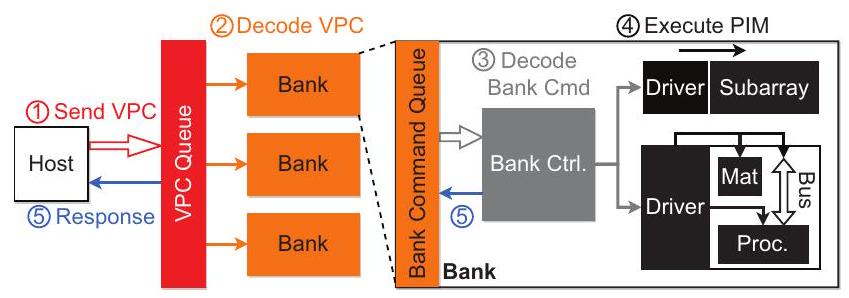
\includegraphics[max width=\textwidth]{2024_05_12_abeba8a85da5b5ec4c7bg-08(1)}
\end{center}

Fig. 14: PIM任务的控制流

作为一种折衷方案,我们采用矢量粒度,其中主机PIM命令指示要操作的矢量。这种设计使得解码过程不那么复杂,在矩阵乘法中命令数量降低到$O(n^2)$,同时保留了足够的主机可编程性。我们定制的PIM命令称为矢量处理命令(VPC)。表II给出了我们使用的不同VPC的描述。主要类型的矩阵计算可以通过这些VPC的组合来解决,包括加法、矩阵乘法和矩阵-标量乘法。

\section*{B. PIM 控制流}
图 14 描述了 PIM 计算任务的控制流程。从主机发送命令到硬件执行,经历了五个步骤。首先,主机发送 PIM VPC(向量处理命令)到 StreamPIM 设备(1)。然后,这些命令被解码并分发到相关的 bank 和 subarray,然后由 RM 总线和处理器执行(2)、(3)和(4)。执行完成后,会向主机发送响应消息(5)。

VPC 发送和响应。在执行 PIM 任务的过程中,主机不断地向 StreamPIM 设备发送 VPC。为了充分利用多 bank 架构的并行性,命令以异步发送-响应的方式发送,这在关于 DRAM 和 NVM 系统的先前研究中已经探索过。来自主机的输入命令在 StreamPIM 设备内部的 VPC 队列中被缓冲。在一个 VPC 完成执行后,会向主机发送一个响应消息。这种异步设计允许设备同时在不同的 bank 上执行 VPC,从而高效地利用了多 bank 架构。

VPC 解码和分发。在接收到一个 VPC 后,StreamPIM 设备将其解码为一个或多个 bank 命令,如图 14 所示。具体来说,为了避免在 subarray 之间进行中间结果的不必要数据移动,一个 VPC 在单个 subarray 内执行。因此,如果向量操作数和结果都在单个 bank 的地址范围内,则 VPC 直接发送到目标 bank。否则,将会向相应的 bank 发送若干个读/写命令,以准备好数据。这些命令收集向量操作数并将它们发送到处理器中的特定 bank。之后,结果通过读/写命令保存到目标 bank 中。

为了在 subarray 上执行 bank 命令,bank 控制器将命令解码为操作,并管理驱动器在 RM 总线和 RM 处理器上执行它们。例如,一个向量点积命令被解码为:(1)两个数据传输操作,从 RM mats 中提取向量操作数到 RM 处理器;(2)一组标量乘法操作;

\begin{center}
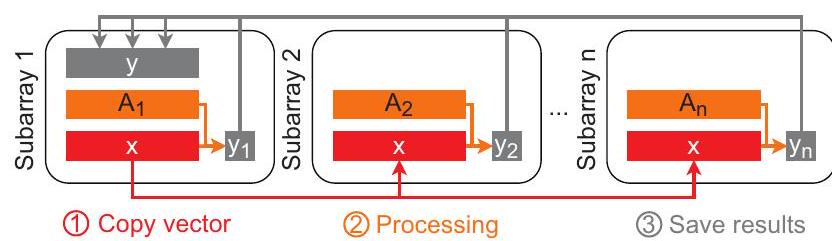
\includegraphics[max width=\textwidth]{2024_05_12_abeba8a85da5b5ec4c7bg-08}
\end{center}


图 15:分布式执行示例。

(3)一组标量加法操作,将标量乘法的结果相加以生成最终结果;(4)数据传输操作,将结果存储到目标 mat。类似于 VPC 解码,如果操作数位于不同的 subarray 中,将生成若干个读/写操作来获取操作数并存储结果。
\section*{C. 并行优化}

子阵列级并行性。由于一个VPC由单个RM处理器执行,性能受到设备时钟频率的限制。为了缓解这种影响,我们提出了一种定制的矩阵计算数据放置方法。以$y=A x$的执行为例,其中$x, y$是$n$维向量,$A$是一个$n * n$矩阵。整个任务被解决为$n$个VPC,作为$x$和$A$中不同行之间的点积,表示为$y_{1}=A_{1} x, y_{2}=A_{2} x, \ldots, y_{n}=A_{n} x$。一个简单的基础方法是将不同的行放置在连续的地址上。因此,一个子阵列负责执行多个$y_{i}=A_{i} x$ VPCs。由于一个子阵列只包含一个处理器,这些VPCs将被串行执行,这会损害并行性并降低性能。为了解决这个问题,我们提出了一个分布式方法,如图15所示。$A$的不同行存储在不同的子阵列中。在数据处理之前,StreamPIM通过子阵列和银行间的通信,通过将$x$复制到不同的子阵列中(1)来执行额外的数据准备。然后,可以在这些子阵列上同时执行不同的$y_{i}=A_{i} x$ VPCs(2)。不同子阵列产生的结果然后被收集并传输到包含$y$的目标子阵列中(3)。在矩阵乘法的情况下(例如,$A * B$),分布式优化将计算分解为多个矩阵-向量乘法(例如,$A * B_{i}$,其中$B_{i}$是$B$的列)。然后,它使用上述优化来执行$A * B_{i}$的计算。在执行$A * B_{i}$期间,分布式将根据需要将$B_{i}$复制到不同的子阵列中,其中$A$的行存储,进行向量点积,并收集结果。

分布式优化将VPC中的向量长度限制为可以完全放置在单个子阵列中的长度。在大多数情况下,这是可以实现的,因为我们设计的子阵列具有较大的内存容量(在我们的实验中,仅为总内存容量的$1/2048$)。为了处理大于子阵列容量的超大向量,StreamPIM采用了切片策略[14],[65],将向量的不同部分分配到不同的子阵列中,处理它们,然后收集结果。

减轻操作阻塞。执行分布式优化需要对数据进行必要的子阵列和银行间的数据复制,以将向量分发到不同的子阵列中。

\begin{verbatim}
task = create_pim_task() // Step 1
// A, B, C are pre-allocated arrays
task.add matrix(A, size1, size2) // Step 2
task.add_matrix(B, size2, size3)
task.add matrix(C, size1, size3)
task.add-operation(MUL, A, B, C)
task.run()
// Step 3
\end{verbatim}


图16: 编程接口示例。

这种复制主要通过读/写操作进行,而子阵列内的传输和计算则通过RM移位操作进行。然而,为了数据的完整性,移位操作不能与单个子阵列中的读/写操作同时执行。因此,当一个子阵列正在执行计算时,针对该子阵列的读/写操作将被阻塞。此外,需要来自这些读/写操作的数据的其他子阵列上的计算也将被阻塞。因此,不同子阵列上的计算被串行化,损害了并行性并降低了整体性能。

为了解决这个问题,我们提出了一种称为"解除阻塞"的方法。首先,在单个矩阵计算任务中,操作数和结果被放置在不重叠的预定义子阵列集中。通过这种布局优化,一个矩阵计算任务的读/写和计算操作被解耦为不同的子阵列集,减轻了这些操作之间的阻塞。其次,重新排列计算和读/写操作的执行顺序,使它们交错访问不同的子阵列。通过这样做,计算和读/写操作不会在同一个子阵列上相互阻塞。这也减轻了在银行命令之间的操作阻塞。通过分布和解除阻塞优化,可以充分利用子阵列级并行性,提高整体性能。

\section*{D. 编程接口}

为了弥合矩阵级任务和向量级命令之间的差距,我们提出了一套编程接口,并将它们作为运行时库提供。

通常,编程一个 StreamPIM 任务需要三个步骤。图 16 显示了一个示例。在第一步中,创建一个 PIM 任务。从概念上讲,任务处理一组矩阵操作数(源和目标)和计算操作。这些操作数和操作期望彼此相互依赖,因此将它们优化为一个整体过程是有益的。程序员可以通过接口告知任务精确的操作数和操作(第二步)。任务然后通过使用第 IV-C 节中描述的优化策略来确定具体的优化策略。在图 16 中显示的示例中,当矩阵相加时(第 3-5 行),通过分布和解除阻塞提出的布局优化,任务确定这些矩阵的向量在计算过程中需要分布到的子阵列。这个布局优化使用了 TRAN VPCs(参见表 II)来执行必要的复制操作。

\begin{center}
\begin{tabular}{|c|c|}
\hline
Processor & 16 cores, X86 ISA, 3.7 GHz, out-of-order \\
\hline
Cache & $512 \mathrm{KiB}$ L1-cache, 8 MiB L2-cache \\
\hline
DW memory & \begin{tabular}{c}
$8 \mathrm{GiB} ; 2400 \mathrm{MHz}$ IO bus speed \\
bank-subarray-mat: $32-64-16 ; 256 \mathrm{KiB} / \mathrm{mat}$ \\
\end{tabular} \\
\hline
core frequency: $100 \mathrm{MHz}$ &  \\
StreamPIM & \begin{tabular}{c}
copos \\
in-processor duplicator count: 2 \\
save track/transfer track: $512 / 512$ (per mat) \\
latency: read: 3.91 write: 10.27 shift: 2.13 (ns) \\
energy: read: 3.80 write: 11.79 shift: 3.26 (pJ) \\
PIM energy: add: 0.03 mul: 0.18 (pJ) \\
fabrication process: $32 \mathrm{~nm}$ \\
\end{tabular} \\
\hline
\end{tabular}
\end{center}

表III: CPU 和内存配置

\begin{center}
\begin{tabular}{|cccc|}
\hline
Benchmark & Process task & \#PIM-VPC & \#move-VPC \\
\hline
$2 \mathrm{~mm}$ & $E=\alpha A B C+\beta D$ & $7.37 \times 10^{6}$ & $7.36 \times 10^{6}$ \\
$3 \mathrm{~mm}$ & $G=(A B)(C D)$ & $1.19 \times 10^{7}$ & $1.18 \times 10^{7}$ \\
gemm & $C^{\prime}=\alpha A B+\beta C$ & $4.61 \times 10^{6}$ & $4.60 \times 10^{6}$ \\
syrk & $C^{\prime}=\alpha A A^{T}+\beta C$ & $6.77 \times 10^{6}$ & $6.76 \times 10^{6}$ \\
syr2k & $C^{\prime}=\alpha A B^{T}+\alpha B A^{T}+\beta C$ & $1.36 \times 10^{7}$ & $1.35 \times 10^{7}$ \\
atax & $y=A^{T} A x$ & $4.00 \times 0^{3}$ & $8.40 \times 10^{3}$ \\
bicg & $q=A p, s=A^{T} r$ & $3.60 \times 10^{3}$ & $8.00 \times 10^{3}$ \\
gesu & $y=\alpha A x+\beta B x$ & $5.60 \times 10^{3}$ & $8.40 \times 10^{3}$ \\
mvt & $x_{1}=x_{1}+A y_{1}, x_{2}=x_{2}+A^{T} y_{2}$ & $8.00 \times 10^{3}$ & $1.60 \times 10^{4}$ \\
\hline
\end{tabular}
\end{center}

表 IV: 工作负载特征。

当操作被添加时(第6行),任务决定了计算所需的VPC,并通过unblock方法重新排列所有VPC的顺序。由于优化策略会随着在第2步中持续添加操作数和操作而不断调整,直到调用task.run()时(表示任务已稳定),实际的计算才会执行。基于优化策略,任务进行布局优化,并按优化后的顺序生成VPC以执行计算(第3步)。

\section*{V. 评估}
\section*{A. 实验设置}
方法学。为了探索RM启用系统的全部设计空间,我们将现有的主存储系统在全系统模拟器gem5中替换为RM延迟模型。延迟模型是从流行的NVM内存建模工具(RTSim和NVSim)中衍生出来的。为了精确模拟RM中的PIM延迟,我们从头开始构建了一个周期精确的模拟器。我们的模拟器采用了基于实验室环境中的真实研究样本推导出的域墙逻辑结构模型。表III列出了我们实验中CPU平台和域墙内存的详细配置。具体来说,我们采用了一个16核的X86处理器和一个8GB的域墙内存。域墙内存被组织成32个bank,包括8个PIM bank和24个内存bank。每个PIM bank集成了用于执行矩阵计算的RM处理器子阵列,而内存bank则仅用于内存请求。我们根据现有研究[18] [46]将内存核心频率设置为100MHz,以保证我们设计中所有流水线组件的功能。我们采用了来自先前工作[26] [82]的RM能耗配置,并通过参考真实的研究样本[46]来推导我们的RM处理器的能耗统计数据。

计算平台。我们设置了6个不同的计算平台进行评估:(1) CPU-RM:采用CPU和RM的传统计算平台;

\begin{center}
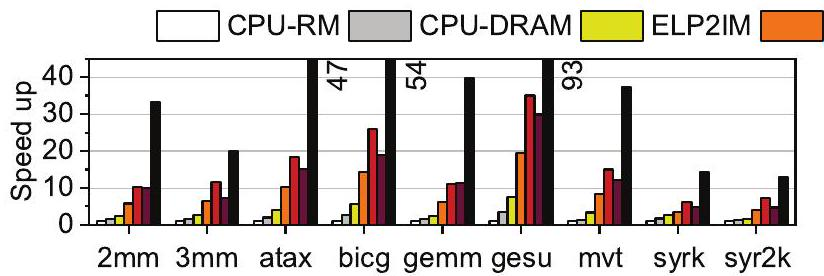
\includegraphics[max width=\textwidth]{2024_05_12_abeba8a85da5b5ec4c7bg-10(1)}
\end{center}

图17:与CPU-RM相比的性能加速。

\begin{center}
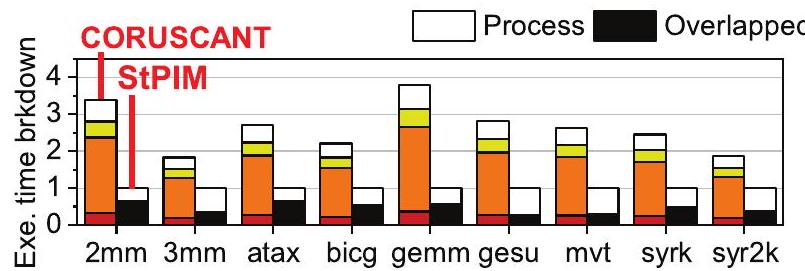
\includegraphics[max width=\textwidth]{2024_05_12_abeba8a85da5b5ec4c7bg-10(3)}
\end{center}

图 19: 相对于StPIM的执行时间分解。

(2) CPU-DRAM: 传统的计算平台,采用CPU和DDR4 DRAM,IO速度为 $2400 \mathrm{MHz}$;
(3) StPIM: StreamPIM(简称为StPIM)平台,具有 512 个 PIM 子阵列,并采用第 IV 节中提出的优化方案(即分发和解除阻塞);
(4) StPIM-e: 类似于 StPIM,但子阵列内的 RM 总线被传统的电气总线替换,这有助于分析 RM 总线的效率;
(5) ELP2IM: 实现了最先进的基于 DRAM 进程的工作 [78],通过串行比特级逻辑操作执行算术运算;
(6) FELIX: 实现了最先进的基于 NVM 进程的工作 [19],通过串行比特级逻辑操作执行算术运算;
(7) CORUSCANT: 实现了最先进的基于 RM 进程的工作 [53]。
请注意,我们在 ELP2IM、FELIX、CORUSCANT 和 StreamPIM 中设置了相同的配置,包括内存核心频率和领域壁纳米线的制造工艺(参见表 III)。我们还忽略了 ELP2IM、FELIX 和 CORUSCANT 中的子阵列间和银行间数据移动的成本,以使它们成为理想情况。所有平台都忽略了错误容忍支持的成本,以保证公平性。

工作负载。为了定量评估我们的设计在矩阵计算上的性能,我们从 polybench [59] 中选择了 9 个代表性的工作负载,涵盖了广泛的线性代数应用 [9], [83]。评估的工作负载的详细信息列在表 IV 中。请注意,表 IV 和后续的图表中,gesu 是 gesummv 的缩写。这些工作负载包括不同的矩阵处理操作,包括矩阵、向量和标量的加法和乘法。为了更好地说明我们的设计在大型数据集上的能力,我们将向量维度设置为 2000,这是 polybench 中的常见配置。对于架构模拟,我们通过修改 polybench 的源代码并将其适配到第 IV 节中提出的优化方案以及第 IV-D 节中讨论的编程接口中,为每个工作负载生成了 VPC 跟踪。我们的循环精确模拟器然后从这些跟踪中提取所有与 VPC 相关的信息并对其进行处理。表 IV 中的 #PIM-VPC 和 #move-VPC 列分别表示每个跟踪中的处理和数据移动的 VPC 计数。

\begin{center}
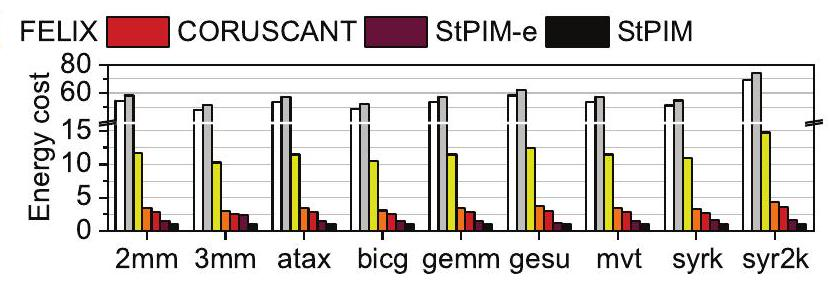
\includegraphics[max width=\textwidth]{2024_05_12_abeba8a85da5b5ec4c7bg-10}
\end{center}

Fig. 18: 能耗成本(标准化为 StPIM)

\begin{center}
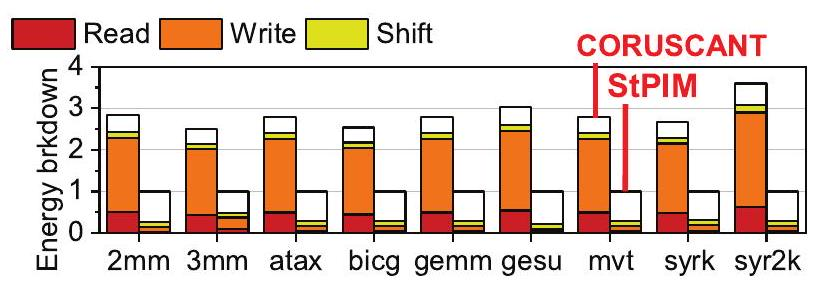
\includegraphics[max width=\textwidth]{2024_05_12_abeba8a85da5b5ec4c7bg-10(2)}
\end{center}

Fig. 20: 能耗成本细分(标准化为 StPIM)

\section*{B. 总体性能}

图17显示了不同计算平台在各种工作负载下的性能,以相对于CPU-RM的加速比表示。我们提供了CPU-DRAM的性能,以更好地说明基于RM的架构的绝对性能。具体而言,由于具有较短的访问延迟和更高的带宽,CPU-DRAM的性能平均提高了1.5倍,超过了CPU-RM。 StPIM-e通过有效地消除PIM技术中的数据传输开销,相比CPU-RM平均提高了12.7倍的速度。此外,分布和解除阻塞优化有助于充分利用子阵列级并行性,从而实现了显著的性能提升。 StPIM通过利用内部RM总线成功降低了RM材料和处理器之间的数据传输开销。这些开销通过RM总线的流水线传输进一步隐藏。因此,相对于StPIM-e和CPU-RM,StPIM的性能分别提高了3.1倍和39.1倍。另一方面,虽然理想的CORUSCANT解决方案相对于CPU-RM基线有15.6倍的性能,但StPIM的平均超过了CORUSCANT 2.5倍。这是因为StPIM可以通过流水线架构摊销标量操作的执行开销,而CORUSCANT受到较重的数据转换开销的影响,导致执行时间较长。由于ELP2IM仅支持位级逻辑操作,其算术运算的性能受到串行位级逻辑操作的限制,限制了其内部并行性。因此,相对于CPU-RM基线,ELP2IM仅实现了3.6倍的加速。 FELIX通过在NVM上执行计算,消除了DRAM所需的预充电阶段,并将性能提高到CPU-RM的8.7倍。但是,FELIX的性能仍然受到串行位级操作的限制。相反,CPRUSCANT和StPIM相对于FELIX分别提高了1.8倍和4.5倍,并相对于ELP2IM分别提高了4.4倍和10.9倍。

图19显示了CORUSCANT和StPIM的执行时间细分,将其标准化为StPIM。执行时间分为独占数据传输时间

\begin{center}
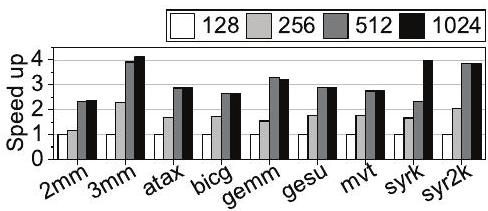
\includegraphics[max width=\textwidth]{2024_05_12_abeba8a85da5b5ec4c7bg-11}
\end{center}

图21:不同PIM子阵列数量的性能。

\begin{center}
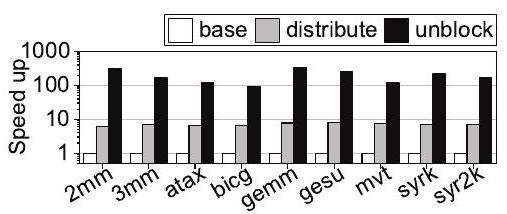
\includegraphics[max width=\textwidth]{2024_05_12_abeba8a85da5b5ec4c7bg-11(1)}
\end{center}

图22:不同优化方案的性能。(包括读取、写入和移位),独占处理时间(处理)和重叠部分(重叠)。对于CORUSCANT,读取、写入和移位分别表示RM读取、写入和移位操作的执行时间。对于StPIM,移位表示子阵列内的数据传输开销,而写入和读取表示子阵列间和银行间的数据移动开销。结果显示,CORUSCANT受到了大量的数据传输开销(平均为 $81.82 \%$).相比之下,通过以流水线方式执行数据传输和处理,StPIM将传输时间隐藏在处理时间中,将独占数据传输开销降低到$1.0\%$以下。

\section*{C. 能量消耗}
图18显示了不同平台的平均能耗,将其标准化为StPIM。由于存储设备(即DRAM和RM)的能耗相对较低,比计算单元和数据传输过程要少,基于DRAM的架构(CPU-DRAM)的能耗接近于基于RM的架构(CPU-RM)。通过消除在内存和计算单元之间传输数据的能耗密集型过程,StPIM相比于CPU-DRAM基准线实现了58.4倍的能效提升。与FELIX和CORUSCANT相比,StPIM的能效分别提高了3.5倍和2.8倍。这是因为StPIM主要通过能效高的移位操作执行数据传输和处理,而FELIX和CORUSCANT依赖于电磁转换操作(即读取和写入),这些操作消耗更多能量。与ELP2IM相比,StPIM的能效提高了11.7倍,因为它消除了DRAM技术所需的耗能刷新和预充电操作。此外,由于RM处理器的能耗比基于CMOS的单元更低,StPIM-e相比于FELIX和CORUSCANT分别提高了2.2倍和1.8倍。然而,由于电气总线的能效低于RM总线,StPIM-e的能耗平均比StPIM多1.6倍。

图20显示了CORUSCANT和StPIM的能量成本细分,标准化为StPIM。由于StPIM通过移位操作而不是电磁转换来传输数据,StPIM中数据传输的平均能量分数仅为30%。相比之下,由于电磁转换操作效率低下,CORUSCANT的能源开销平均增加了86%。








\section*{D. 敏感性测试}

PIM子阵列数量。我们通过调整每个银行的子阵列数量和每个子阵列的内存容量来评估PIM对StPIM性能的影响。






\begin{center}
\begin{tabular}{|c|c|c|c|c|}
\hline
Segment size & 64 & 256 & 512 & 1024 \\
\hline
Execution time & $+2.33 \%$ & $+0.58 \%$ & $+0.29 \%$ & $0 \%$ \\
\hline
Energy cost & $-0.1 \%$ & $-0.05 \%$ & $-0.04 \%$ & $0 \%$ \\
\hline
\end{tabular}
\end{center}

表格V: 不同总线段大小之间的平均性能和能耗比较(标准化为1024)。

图21展示了性能结果,其标准化为128个子阵列基线(128)。与基线相比,使用256、512和1024个子阵列可以将平均性能提高$1.74 \times, 3.0 \times$和$3.2 \times$,分别。随着子阵列数量的增加,平均性能有望达到饱和,因为数据依赖性限制了更高的并行性。

优化。我们通过选择性地应用分布和解锁优化来评估它们的好处。图22显示了相对于基线(即无优化)标准化的结果。基线的性能受到低内存核心频率和RM内部并行性利用不足的限制。采用分布优化比基线平均提高了$7.1 \times$的性能。这是因为分布可以通过在不同的子阵列之间分配计算来更好地利用子阵列级并行性。然而,分布的性能仍然受到操作阻塞的限制。通过成功解决这个问题,解锁比基线平均提高了$199.7 \times$的性能。

段大小。由于RM总线以段的形式传输数据,段大小影响传输性能。由于数据只能在一个周期内由一个段传输,缩小段大小会增加RM总线上的段数,需要更多的周期在RM阵列和处理器之间传输数据。然而,由于在大多数周期中,总线传输与计算同时进行并且其开销被隐藏起来(参见第V-B节),因此这种影响是微小的。表V给出了敏感性测试结果。将段大小从1024缩小到64仅会对总体性能产生$2.33\%$的平均开销。另一方面,增加段大小会导致更多的能量消耗,因为电流更大。然而,由于段数减少,从而减少了移位操作的数量,这种能量开销得到了补偿。因此,能量成本几乎保持不变,如表V所示。在我们的评估中,我们选择1024作为默认设置,以展示我们设计的最佳性能。

\section*{E.端到端性能}
为了展示端到端性能,我们将两个深度神经网络应用程序改进为 StreamPIM,包括 MLP(多层感知器)[41] 和 BERT [16]。由于这些 DNN 应用程序包含各种类型的计算操作,我们只将矩阵乘法和加法转移到 StreamPIM 上,而依靠 CPU 处理不支持的操作(即非线性操作)。图 23 描述了各种计算平台相对于 CPU-DRAM 的执行速度提升。由于 MLP 中的非线性层只占 MLP 推断的一小部分,StreamPIM 通过显著加速矩阵计算,相比 CPU-DRAM 实现了 54.77 倍的速度提升。此外,与 CORUSCANT 相比,StreamPIM 的性能提高了 1.86 倍,这归功于其针对矩阵操作的特定优化。另一方面,由于 BERT 包含更多的非线性操作(例如,矩阵归一化),StreamPIM 显示出相对较少的性能增益。然而,通过加速 BERT 推断中的关键矩阵计算部分,StreamPIM 仍然实现了比 CPU-DRAM 和 CORUSCANT 分别高出 4.49 倍和 1.97 倍的性能。

\section*{F. 制造过程}
由于StreamPIM中的所有算术操作都是通过移位操作执行的,能量成本主要由移位电流水平和制造工艺决定,并通过公式和从研究中得出的统计数据进行计算。当域尺度缩小时,每个门的能量成本会急剧降低。例如,当域尺度从$1.0\mu \mathrm{m}$缩小到$32 \mathrm{~nm}$时,每个门的能量成本将从$20 \mathrm{pJ}$下降到$0.0008 \mathrm{pJ}$。在我们的评估中,我们采用了CORUSCANT兼容的配置(即$32 \mathrm{~nm}$),在这种配置下,加法和乘法操作的能量消耗分别为$0.03 \mathrm{pJ}$和$0.18 \mathrm{pJ}$,与基于CMOS的算术单元相比,显示出了出色的能量效率。

\section*{G. 面积开销}
我们通过估算不同组件中域壁存储单元(RM mats)的数量来分析我们设计的面积分布情况。每个子阵列中域壁存储单元的数量、总的 PIM 子阵列数量以及总的子阵列数量的配置是性能和面积开销之间的权衡。在我们的默认配置中,我们假设每个子阵列包含 16 个 RM mats,其中有 2 个 mats 有传输轨道。此外,我们假设有 512 个 PIM 子阵列和 2048 个总的子阵列。RM 总线和 RM 处理器仅占 RM 设备总面积的 $1.8 \%$ 和 $0.1 \%$。另一方面,传输轨道的面积开销仅为总面积的 $3.1 \%$,而添加的控制逻辑的面积开销与根据之前的研究[82]的银行面积相比仅约为 $1.0 \%$。结果表明,我们的设计在性能和面积消耗之间取得了良好的平衡。

\section*{VI. RELATED WORKS AND DISCUSSION}
PCRAM和STT-MRAM中的PIM。许多先前的工作已经提出了基于PCRAM和STTMRAM的PIM架构。例如,一个典型的基于PCRAM的处理架构,Pinatubo [43],同时打开两个内存行,并通过调整的阈值电压感测它们,以执行位逻辑操作。另一项工作 [31] 在STT-MRAM中提出了类似的方法。其他研究 [6], [19], [21] 提出了单元内的布尔运算,以避免添加复杂的感测电路。这些方法只能支持位逻辑操作(例如,AND和OR)。因此,一个算术操作需要多个步骤,产生大量的中间结果,并生成大量的内存读写。相比之下,由于StreamPIM采用定制的算术单元来支持高级算术操作,例如加法、乘法和点积,因此它显著减少了矩阵计算过程中的中间结果数量。交叉点ReRAM中的PIM。作为处理内ReRAM架构的典型实现,交叉点设计 [14], [65], [70] 能够执行矢量点积。在交叉点架构中,一列单元中的数据和位线上的输入电压被视为两个矢量操作数。然后,字线上的电流将形成这两个矢量的点积。此外,使用MLC(多级单元)技术,一个单元可以存储多个位,输入电压也可以调整到多个级别。因此,交叉点点积可以获得更高的精度。基于交叉点的PIM架构可以实现高吞吐量和能效。然而,MLC方法 [14] 需要进行必要的模数转换(ADC),这带来了不可忽视的开销。与此同时,SLC(单级单元)设计 [70] 只能支持基本的位级操作,需要多个步骤和大量的中间结果来执行高级计算。相比之下,StreamPIM 可以通过将数据存储和处理为数字形式来消除ADC开销,并支持高级算术操作以减少中间步骤和结果的数量。

硬件实现。作为一种新提出的技术,将基于域壁的处理器投入大规模生产仍然需要多个步骤。一个关注点是处理器的可靠性。在概念验证实验中,几个级联电路展示了良好的可靠性 [46]。还有几项工作提出了改善DMI可靠性的方法 [44], [75]。另一个关注点是RM总线,主要受到移位故障的影响。多项工作已经成功地缓解了甚至避免了移位故障问题 [35], [54]。StreamPIM可以利用这些方法从物理/材料角度提高其硬件可靠性。此外,StreamPIM 还可以采用[53] 中的架构支持(即冗余设计)来补偿误差容限。

支持的操作。在本文中,StreamPIM专注于加速数据密集型和计算密集型应用中最基本的操作(即加法和乘法)。为了支持这些操作,StreamPIM基于逻辑门从头开始构建了定制的加法器和乘法器。通过实现和集成其他指定的处理器(例如,除法器、平方根提取器和浮点处理器 [5], [29], [32], [52], [76], [81]),StreamPIM可以扩展到支持更多的算术操作和数据表示类型。这些扩展可以使StreamPIM适用于更广泛的计算内核(例如,FFT和DNN训练)。由于本工作的主要目的是针对处理器内处理的架构设计和优化,因此上述扩展的实现细节,需要专门的设计和优化,由于空间限制而被省略,并留给将来的工作。

编程接口和设备控制。在评估的应用程序中,源代码定义了矩阵级任务,而我们的StreamPIM设备执行标量级计算。为了弥合应用程序源代码和RM设备上的计算之间的差距,StreamPIM提出了一个位于这两个级别之间的向量级接口水平,这在第四节中进行了讨论。在意识到学术和工业领域中以前的工作 [4], [14], [66] 的基础上,StreamPIM选择将这个接口级别作为一套库(包括代码编译器和设备驱动程序)提供。这种设计赋予了接口级别能力:(1)从应用程序中提取计算图并决定优化策略,包括数据放置优化和命令重排序,以及(2)将计算和优化转换为设备级别(即物理)表示并执行它们。

\section*{VII. ConClusion}
我们提出了StreamPIM,一种新的赛道存储器内处理设计,极大地提高了矩阵计算任务的性能和能源效率。StreamPIM直接利用域壁纳米线构建矩阵处理器,从而使赛道存储器能够同时处理计算和I/O任务。它还集成了基于域壁纳米线的总线,以消除转换开销。我们的评估结果表明,与最先进的赛道存储器内处理解决方案相比,StreamPIM实现了性能加速和节能。

\section*{ACKNOWLEDGEMENT}
我们感谢匿名审稿人的建设性反馈。我们感谢Ran带来的所有欢乐。本工作主要得到了中国国家重点研发计划资助(项目编号:2023YFB4502702)、中国国家自然科学基金资助(项目编号:62332021)、以及北京大学基础研究基金资助。李博士部分得到中国国家自然科学基金资助(项目编号:62202396)。罗博士部分得到中国国家重点研发计划资助(项目编号:2022YFA1203904)和中国国家自然科学基金资助(项目编号:52271160)。孙博士部分得到中国国家自然科学基金资助(项目编号:62032001)。通讯作者为Jie Zhang.

\section*{REFERENCES}
[1] "Amd ryzen"TM 9 5950x desktop processors," \href{https://www.amd.com/en/}{https://www.amd.com/en/} products/cpu/amd-ryzen-9-5950x, 2020.

[2] "Geforce rtx 3080 family," \href{https://www.nvidia.com/en-us/geforce/}{https://www.nvidia.com/en-us/geforce/} graphics-cards/30-series/rtx-3080-3080ti/, 2021.

[3] M. Abadi, P. Barham, J. Chen, Z. Chen, A. Davis, J. Dean, M. Devin, S. Ghemawat, G. Irving, M. Isard, M. Kudlur, J. Levenberg, R. Monga, S. Moore, D. G. Murray, B. Steiner, P. A. Tucker, V. Vasudevan, P. Warden, M. Wicke, Y. Yu, and X. Zhang, "Tensorflow: A system for large-scale machine learning," ArXiv, vol. abs/1605.08695, 2016.\\
[4] N. Agarwal, D. W. Nellans, M. W. Stephenson, M. O'Connor, and S. W. Keckler, "Page placement strategies for gpus within heterogeneous memory systems," Proceedings of the Twentieth International Conference on Architectural Support for Programming Languages and Operating Systems, 2015. [Online]. Available: \href{https://api.semanticscholar.org/CorpusID:207221462}{https://api.semanticscholar.org/CorpusID:207221462}

[5] M. Anas, R. S. Padiyar, and A. S. Boban, "Implementation of cordic algorithm and design of high speed cordic algorithm," 2017 International Conference on Energy, Communication, Data Analytics and Soft Computing (ICECDS), pp. 1278-1281, 2017. [Online]. Available: \href{https://api.semanticscholar.org/CorpusID:49341209}{https://api.semanticscholar.org/CorpusID:49341209}

[6] S. Angizi, Z. He, A. Awad, and D. Fan, "Mrima: An mram-based inmemory accelerator," IEEE Transactions on Computer-Aided Design of Integrated Circuits and Systems, vol. 39, pp. 1123-1136, 2020.

[7] I. I. Arikpo, F. U. Ogban, and I. E. Eteng, "Von neumann architecture and modern computers," Global Journal of Mathematical Sciences, vol. 6, pp. $97-103,2008$.

[8] N. N. Baharudin, R. A. Alsaqour, H. Shaker, M. S. Abdelhaq, O. Alsaqour, and T. Alahdal, "Review on multiplexing techniques in bandwidth utilization," Middle-East Journal of Scientific Research, vol. 18, pp. $1510-1516,2013$

[9] W. Bao, S. Krishnamoorthy, L.-N. Pouchet, F. Rastello, and P. Sadayappan, "Polycheck: dynamic verification of iteration space transformations on affine programs," Proceedings of the 43rd Annual ACM SIGPLANSIGACT Symposium on Principles of Programming Languages, 2016.

[10] N. Binkert, B. Beckmann, G. Black, S. K. Reinhardt, A. Saidi, A. Basu, J. Hestness, D. R. Hower, T. Krishna, S. Sardashti, R. Sen, K. Sewell, M. Shoaib, N. Vaish, M. D. Hill, and D. A. Wood, "The gem5 simulator," SIGARCH Comput. Archit. News, vol. 39, no. 2, p. 1-7, aug 2011. [Online]. Available: \href{https://doi.org/10.1145/2024716.2024718}{https://doi.org/10.1145/2024716.2024718}

[11] T. B. Brown, B. Mann, N. Ryder, M. Subbiah, J. Kaplan, P. Dhariwal, A. Neelakantan, P. Shyam, G. Sastry, A. Askell, S. Agarwal, A. HerbertVoss, G. Krueger, T. J. Henighan, R. Child, A. Ramesh, D. M. Ziegler, J. Wu, C. Winter, C. Hesse, M. Chen, E. Sigler, M. Litwin, S. Gray, B. Chess, J. Clark, C. Berner, S. McCandlish, A. Radford, I. Sutskever, and D. Amodei, "Language models are few-shot learners," ArXiv, vol. $\mathrm{abs} / 2005.14165,2020$.

[12] G. W. Burr, M. J. Breitwisch, M. M. Franceschini, D. Garetto, K. Gopalakrishnan, B. L. Jackson, B. N. Kurdi, C. H. Lam, L. A. Lastras, A. Padilla, B. Rajendran, S. Raoux, and R. S. Shenoy, "Phase change memory technology," Journal of Vacuum Science \& Technology. B. Nanotechnology and Microelectronics: Materials, Processing, Measurement, and Phenomena, vol. 28, pp. 223-262, 2010.

[13] S. Catalán, J. González-Domínguez, R. Mayo, and E. S. QuintanaOrtí, "Analyzing the energy efficiency of the memory subsystem in multicore processors," 2014 IEEE International Symposium on Parallel and Distributed Processing with Applications, pp. 10-17, 2014.

[14] P. Chi, S. Li, C. Xu, T. Zhang, J. Zhao, Y. Liu, Y. Wang, and Y. Xie, "Prime: A novel processing-in-memory architecture for neural network computation in reram-based main memory," 2016 ACM/IEEE 43rd Annual International Symposium on Computer Architecture (ISCA), pp. 27-39, 2016.

[15] J.-H. Choe, "Memory technology 2021: Trends \& challenges," 2021 International Conference on Simulation of Semiconductor Processes and Devices (SISPAD), pp. 111-115, 2021. [Online]. Available: \href{https://api.semanticscholar.org/CorpusID:243916892}{https://api.semanticscholar.org/CorpusID:243916892}

[16] J. Devlin, M.-W. Chang, K. Lee, and K. Toutanova, "Bert: Pre-training of deep bidirectional transformers for language understanding," ArXiv, vol. $a b s / 1810.04805,2019$.

[17] X. Dong, X. Wu, G. Sun, Y. Xie, H. H. Li, and Y. Chen, "Circuit and microarchitecture evaluation of 3d stacking magnetic ram (mram) as a universal memory replacement," 2008 45th ACM/IEEE Design Automation Conference, pp. 554-559, 2008.

[18] X. Dong, C. Xu, Y. Xie, and N. P. Jouppi, "Nvsim: A circuit-level performance, energy, and area model for emerging nonvolatile memory," IEEE Transactions on Computer-Aided Design of Integrated Circuits and Systems, vol. 31, pp. 994-1007, 2012.

[19] S. Gupta, M. Imani, and T. Simunic, "Felix: Fast and energy-efficient logic in memory," 2018 IEEE/ACM International Conference on ComputerAided Design (ICCAD), pp. 1-7, 2018.

[20] A. Hansson, N. Agarwal, A. Kolli, T. Wenisch, and A. N. Udipi, "Simulating dram controllers for future system architecture exploration," in 2014 IEEE International Symposium on Performance Analysis of Systems and Software (ISPASS), 2014, pp. 201-210.

[21] Z. He, S. Angizi, and D. Fan, "Accelerating low bit-width deep convolution neural network in mram," 2018 IEEE Computer Society Annual Symposium on VLSI (ISVLSI), pp. 533-538, 2018.

[22] M. Heide, G. Bihlmayer, and S. Blügel, "Dzyaloshinskii-moriya interaction accounting for the orientation of magnetic domains in ultrathin films: Fe/w(110)," Physical Review B, vol. 78, p. 140403, 2008.

[23] S. Hong, T. Oguntebi, and K. Olukotun, "Efficient parallel graph exploration on multi-core cpu and gpu," 2011 International Conference on Parallel Architectures and Compilation Techniques, pp. 78-88, 2011.

[24] M. Horowitz, "1.1 computing's energy problem (and what we can do about it)," 2014 IEEE International Solid-State Circuits Conference Digest of Technical Papers (ISSCC), pp. 10-14, 2014.

[25] M. Hosomi, H. Yamagishi, T. Yamamoto, K. Bessho, Y. Higo, K. Yamane, H. Yamada, M. Shoji, H. Hachino, C. Fukumoto, H. Nagao, and H. Kano, "A novel nonvolatile memory with spin torque transfer magnetization switching: spin-ram," IEEE InternationalElectron Devices Meeting, 2005. IEDM Technical Digest., pp. 459-462, 2005.

[26] Q. Hu, G. Sun, J. Shu, and C. Zhang, "Exploring main memory design based on racetrack memory technology," 2016 International Great Lakes Symposium on VLSI (GLSVLSI), pp. 397-402, 2016.

[27] A. Iyengar and S. Ghosh, "Modeling and analysis of domain wall dynamics for robust and low-power embedded memory," 2014 51st ACM/EDAC/IEEE Design Automation Conference (DAC), pp. 1-6, 2014. [Online]. Available: \href{https://api.semanticscholar.org/CorpusID:233579}{https://api.semanticscholar.org/CorpusID:233579}

[28] H. Jiang, Y. Chen, Z. Qiao, T.-H. Weng, and K.-C. Li, "Scaling up mapreduce-based big data processing on multi-gpu systems," Cluster Computing, vol. 18, pp. 369-383, 2014.

[29] H. Jiang, L. Liu, F. Lombardi, and J. Han, "Adaptive approximation in arithmetic circuits: A low-power unsigned divider design," 2018 Design, Automation \& Test in Europe Conference \& Exhibition (DATE), pp. 14111416, 2018. [Online]. Available: \href{https://api.semanticscholar.org/CorpusID:}{https://api.semanticscholar.org/CorpusID:} 5050678

[30] U. Kang, H. soo Yu, C. Park, H. Zheng, J. B. Halbert, K. Bains, S.-J. Jang, and J.-S. Choi, "Co-architecting controllers and dram to enhance dram process scaling," 2014.

[31] W. Kang, H. Wang, Z. Wang, Y. Zhang, and W. Zhao, "In-memory processing paradigm for bitwise logic operations in stt-mram," IEEE Transactions on Magnetics, vol. 53, pp. 1-4, 2017.

[32] P. Karlstrom, A. Ehliar, and D. Liu, "High performance, low latency fpga based floating point adder and multiplier units in a virtex 4," 2006 NORCHIP, pp. 31-34, 2006. [Online]. Available: \href{https://api.semanticscholar.org/CorpusID:}{https://api.semanticscholar.org/CorpusID:} 18130812

[33] S. W. Keckler, W. J. Dally, B. Khailany, M. Garland, and D. Glasco, "Gpus and the future of parallel computing," IEEE Micro, vol. 31, pp. $7-17,2011$.

[34] A. A. Khan, F. Hameed, R. Bläsing, S. S. P. Parkin, and J. Castrillón, "Rtsim: A cycle-accurate simulator for racetrack memories," IEEE Computer Architecture Letters, vol. 18, pp. 43-46, 2019. [Online]. Available: \href{https://api.semanticscholar.org/CorpusID:85502870}{https://api.semanticscholar.org/CorpusID:85502870}

[35] A. A. Khan, S. Ollivier, F. Hameed, J. Castrillón, and A. K. Jones, "Downshift: Tuning shift reduction with reliability for racetrack memories," IEEE Transactions on Computers, vol. 72, pp. 2585-2599, 2023. [Online]. Available: \href{https://api.semanticscholar.org/CorpusID:257576810}{https://api.semanticscholar.org/CorpusID:257576810}

[36] Y. Kim, "Architectural techniques to enhance dram scaling," 2018.

[37] Y. Kim, R. Daly, J. S. Kim, C. Fallin, J.-H. Lee, D. Lee, C. Wilkerson, K. Lai, and O. Mutlu, "Flipping bits in memory without accessing them: An experimental study of dram disturbance errors," 2014 ACM/IEEE 41st International Symposium on Computer Architecture (ISCA), pp. 361-372, 2014.

[38] Y. Kim, V. Seshadri, D. Lee, J. Liu, and O. Mutlu, "A case for exploiting subarray-level parallelism (salp) in dram," 2012 39th Annual International Symposium on Computer Architecture (ISCA), pp. 368-379, 2012.

[39] H. Y. Lee, Y. S. Chen, P. S. Chen, P. Gu, Y. Hsu, S. M. Wang, W. H. Liu, C. Tsai, S.-S. Sheu, P.-C. Chiang, W. P. Lin, C. H. Lin, W. S. Chen, F. T. Chen, C. Lien, and M.-J. Tsai, "Evidence and solution of over-reset problem for hfox based resistive memory with sub-ns switching speed and high endurance," 2010 International Electron Devices Meeting, pp. 19.7.1-19.7.4, 2010.

[40] M.-J. Lee, Y. soo Park, B. S. Kang, S. Ahn, C. B. Lee, K. Kim, W. Xianyu, G. B. Stefanovich, J.-H. Lee, S. J. Chung, Y. hee Kim, C.-S. Lee, J. bong Park, and I. kyeong Yoo, "2-stack 1d-1r cross-point structure with oxide diodes as switch elements for high density resistance ram applications," 2007 IEEE International Electron Devices Meeting, pp. 771-774, 2007.\\
[41] F. Leisch and E. Dimitriadou, mlbench: Machine Learning Benchmark Problems, 2021, r package version 2.1-3.1.

[42] P. Li, Y. Luo, N. Zhang, and Y. Cao, "Heterospark: A heterogeneous cpu/gpu spark platform for machine learning algorithms," 2015 IEEE International Conference on Networking, Architecture and Storage (NAS), pp. 347-348, 2015.

[43] S. Li, C. Xu, Q. Zou, J. Zhao, Y. Lu, and Y. Xie, "Pinatubo: A processingin-memory architecture for bulk bitwise operations in emerging nonvolatile memories," 2016 53nd ACM/EDAC/IEEE Design Automation Conference (DAC), pp. 1-6, 2016.

[44] H. Lin, N. Xu, D. Wang, L. Liu, X. Zhao, Y. Zhou, X. Luo, C. Song, G. Yu, and G. Xing, "Implementation of highly reliable and energyefficient nonvolatile in-memory computing using multistate domain wall spin-orbit torque device," Advanced Intelligent Systems, vol. 4, 2022. [Online]. Available: \href{https://api.semanticscholar.org/CorpusID:249221388}{https://api.semanticscholar.org/CorpusID:249221388}

[45] B. Liu, S. Gu, M. Chen, W. Kang, J. Hu, Q. Zhuge, and E. H.-M. Sha, "An efficient racetrack memory-based processing-in-memory architecture for convolutional neural networks," 2017 IEEE International Symposium on Parallel and Distributed Processing with Applications and 2017 IEEE International Conference on Ubiquitous Computing and Communications (ISPA/IUCC), pp. 383-390, 2017.

[46] Z. Luo, A. Hrabec, T. P. Dao, G. Sala, S. Finizio, J. Feng, S. Mayr, J. Raabe, P. Gambardella, and L. J. Heyderman, "Current-driven magnetic domain-wall logic," Nature, vol. 579, pp. 214-218, 2020.

[47] Z. Luo, S. Schären, A. Hrabec, T. P. Dao, G. Sala, S. Finizio, J. Feng, S. Mayr, J. Raabe, P. Gambardella, and L. J. Heyderman, "Field- and current-driven magnetic domain-wall inverter and diode," Physical review applied, vol. 15, 2021

[48] P. J. Nair, D. Kim, and M. K. Qureshi, "Archshield: architectural framework for assisting dram scaling by tolerating high error rates," Proceedings of the 40th Annual International Symposium on Computer Architecture, 2013

[49] B. NALE, R. K. RAMANUJAN, M. P. SWAMINATHAN, T. THOMAS, and T. POLEPEDDI, "Memory channel that supports near memory and far memory access," \href{https://patentcenter.uspto.gov/applications/15081164}{https://patentcenter.uspto.gov/applications/15081164}, Apr 2017, patent US20160210251A1.

[50] C. Napoli, G. Pappalardo, E. Tramontana, and G. Zappalá, "A clouddistributed gpu architecture for pattern identification in segmented detectors big-data surveys," Comput. J., vol. 59, pp. 338-352, 2016.

[51] D. Narayanan, M. Shoeybi, J. Casper, P. LeGresley, M. A. Patwary, V. A. Korthikanti, D. Vainbrand, P. Kashinkunti, J. Bernauer, B. Catanzaro, A. Phanishayee, and M. A. Zaharia, "Efficient large-scale language model training on gpu clusters using megatron-lm," Proceedings of the International Conference for High Performance Computing, Networking, Storage and Analysis, 2021

[52] H. Nikmehr, B. J. Phillips, and C.-C. Lim, "A novel implementation of radix-4 floating-point division/square-root using comparison multiples," Comput. Electr. Eng., vol. 36, pp. 850-863, 2010. [Online]. Available: \href{https://api.semanticscholar.org/CorpusID:8703886}{https://api.semanticscholar.org/CorpusID:8703886}

[53] S. Ollivier, S. Longofono, P. Dutta, J. Hu, S. Bhanja, and A. K. Jones, "Coruscant: Fast efficient processing-in-racetrack memories," 2022 55th IEEE/ACM International Symposium on Microarchitecture (MICRO), pp. $784-798,2022$.

[54] S. Ollivier, S. Longofono, P. Dutta, J. Hu, S. Bhanja, and A. K. Jones, "Toward comprehensive shifting fault tolerance for domain-wall memories with piett," IEEE Transactions on Computers, vol. 72, pp. 1095-1109, 2023. [Online]. Available: \href{https://api.semanticscholar.org/CorpusID:250289532}{https://api.semanticscholar.org/CorpusID:250289532}

[55] OpenAI, "Gpt-4 technical report," ArXiv, vol. abs/2303.08774, 2023.

[56] S. S. P. Parkin, "Racetrack memory: A storage class memory based on current controlled magnetic domain wall motion," 2009 Device Research Conference, pp. 3-6, 2009.

[57] X. Peng, M.-C. Yang, H. M. Tsui, C. N. Leung, and W. Kang, "Smart: on simultaneously marching racetracks to improve the performance of racetrack-based main memory," Proceedings of the 59th ACM/IEEE Design Automation Conference, 2022. [Online]. Available: \href{https://api.semanticscholar.org/CorpusID:251744190}{https://api.semanticscholar.org/CorpusID:251744190}

[58] M. Poremba and Y. Xie, "Nvmain: An architectural-level main memory simulator for emerging non-volatile memories," 2012 IEEE Computer Society Annual Symposium on VLSI, pp. 392-397, 2012

[59] L.-N. Pouchet and S. Grauer-Gray, "Polybench: the polyhedral benchmark suite," \href{https://web.cse.ohio-state.edu/}{https://web.cse.ohio-state.edu/} pouchet.2/software/ polybench, 2012.

[60] A. Quamar, A. Deshpande, and J. J. Lin, "Nscale: neighborhood-centric large-scale graph analytics in the cloud," The VLDB Journal, vol. 25, pp. $125-150,2015$.

[61] R. K. RAMANUJAN, G. J. HINTON, and D. J. ZIMMERMAN, "Dynamic partial power down of memory-side cache in a 2-level memory hierarchy," \href{https://patentcenter.uspto.gov/applications/17009245}{https://patentcenter.uspto.gov/applications/17009245}, Nov 2021, patent US11200176B2.

[62] S. Raoux, G. W. Burr, M. J. Breitwisch, C. T. Rettner, Y.-C. Chen, R. M. Shelby, M. Salinga, D. Krebs, S.-H. Chen, H.-L. Lung, and C. H. Lam, "Phase-change random access memory: A scalable technology," IBM J. Res. Dev., vol. 52, pp. 465-480, 2008.

[63] K. A. Roxy, S. Ollivier, A. Hoque, S. Longofono, A. K. Jones, and S. Bhanja, "A novel transverse read technique for domain-wall "racetrack" memories," IEEE Transactions on Nanotechnology, vol. 19, pp. 648-652, 2020.

[64] V. Seshadri, D. Lee, T. Mullins, H. Hassan, A. Boroumand, J. S. Kim, M. A. Kozuch, O. Mutlu, P. B. Gibbons, and T. C. Mowry, "Ambit: In-memory accelerator for bulk bitwise operations using commodity dram technology," 2017 50th Annual IEEE/ACM International Symposium on Microarchitecture (MICRO), pp. 273-287, 2017.

[65] A. Shafiee, A. Nag, N. Muralimanohar, R. Balasubramonian, J. P. Strachan, M. Hu, R. S. Williams, and V. Srikumar, "Isaac: A convolutional neural network accelerator with in-situ analog arithmetic in crossbars," 2016 ACM/IEEE 43rd Annual International Symposium on Computer Architecture (ISCA), pp. 14-26, 2016.

[66] J. A. Stratton, S. S. Stone, , and W. mei W. Hwu, "Mcuda: An efficient implementation of cuda kernels on multi-cores," 2011. [Online]. Available: \href{https://api.semanticscholar.org/CorpusID:16937005}{https://api.semanticscholar.org/CorpusID:16937005}

[67] Y.-K. Suh, H. Ryu, H. Kim, and K. W. Cho, "Edison: A web-based hpc simulation execution framework for large-scale scientific computing software," in 2016 16th IEEE/ACM International Symposium on Cluster, Cloud and Grid Computing (CCGrid), 2016, pp. 608-612.

[68] G. Sun, C. Zhang, H. Li, Y. Zhang, W. Zhang, Y. Gu, Y. Sun, J.-O. Klein, D. Ravelosona, Y. Liu, W. Zhao, and H. Yang, "From device to system: Cross-layer design exploration of racetrack memory," 2015 Design, Automation \& Test in Europe Conference \& Exhibition (DATE), pp. 1018-1023, 2015. [Online]. Available: \href{https://api.semanticscholar.org/CorpusID:5012927}{https://api.semanticscholar.org/CorpusID:5012927}

[69] Z. Sun, W. Wu, and H. H. Li, "Cross-layer racetrack memory design for ultra high density and low power consumption," 2013 50th ACM/EDAC/IEEE Design Automation Conference (DAC), pp. 1-6, 2013. [Online]. Available: \href{https://api.semanticscholar.org/CorpusID:96798}{https://api.semanticscholar.org/CorpusID:96798}

[70] N. Talati, S. Gupta, P. S. Mane, and S. Kvatinsky, "Logic design within memristive memories using memristor-aided logic (magic)," IEEE Transactions on Nanotechnology, vol. 15, pp. 635-650, 2016. [Online]. Available: \href{https://api.semanticscholar.org/CorpusID:14637261}{https://api.semanticscholar.org/CorpusID:14637261}

[71] J. Vandermeulen, B. V. de Wiele, L. Dupré, and B. V. Waeyenberge, "Logic and memory concepts for all-magnetic computing based on transverse domain walls," Journal of Physics D: Applied Physics, vol. 48, 2015.

[72] R. Venkatesan, V. J. Kozhikkottu, C. Augustine, A. Raychowdhury, K. Roy, and A. Raghunathan, "Tapecache: a high density, energy efficient cache based on domain wall memory," in ISLPED '12, 2012.

[73] R. Venkatesan, M. Sharad, K. Roy, and A. Raghunathan, "Dwm-tapestri - an energy efficient all-spin cache using domain wall shift based writes," 2013 Design, Automation \& Test in Europe Conference \& Exhibition (DATE), pp. 1825-1830, 2013. [Online]. Available: \href{https://api.semanticscholar.org/CorpusID:480593}{https://api.semanticscholar.org/CorpusID:480593}

[74] O. Villa, D. R. Johnson, M. O'Connor, E. Bolotin, D. W. Nellans, J. Luitjens, N. Sakharnykh, P. Wang, P. Micikevicius, A. Scudiero, S. W. Keckler, and W. J. Dally, "Scaling the power wall: A path to exascale," SC14: International Conference for High Performance Computing, Networking, Storage and Analysis, pp. 830-841, 2014.

[75] D. Wang, Z. Wang, N. Xu, L. Liu, H. Lin, X. Zhao, S. Jiang, W. Lin, N. Gao, M. Liu, and G. Xing, "Synergy of spin-orbit torque and built-in field in magnetic tunnel junctions with tilted magnetic anisotropy: Toward tunable and reliable spintronic neurons (adv. sci. 30/2022)," Advanced Science, vol. 9, 2022. [Online]. Available: \href{https://api.semanticscholar.org/CorpusID:251349610}{https://api.semanticscholar.org/CorpusID:251349610}

[76] X. Wang, Y. Zhang, Q. Ye, and S. Yang, "A new algorithm for designing square root calculators based on fpga with pipeline technology," 2009 Ninth International Conference on Hybrid Intelligent Systems, vol. 1, pp. 99-102, 2009. [Online]. Available: https: \href{//api.semanticscholar.org/CorpusID:12733172}{//api.semanticscholar.org/CorpusID:12733172}\\
[77] Y. Wang, H. Yu, D. Sylvester, and P. Kong, "Energy efficient in-memory aes encryption based on nonvolatile domain-wall nanowire," 2014 Design, Automation \& Test in Europe Conference \& Exhibition (DATE), pp. 1-4, 2014

[78] X. Xin, Y. Zhang, and J. Yang, "Elp2im: Efficient and low power bitwise operation processing in dram," 2020 IEEE International Symposium on High Performance Computer Architecture (HPCA), pp. 303-314, 2020.

[79] J. J. Yang, M. D. Pickett, X. Li, D. A. A. Ohlberg, D. R. Stewart, and R. S. Williams, "Memristive switching mechanism for metal/oxide/metal nanodevices." Nature nanotechnology, vol. 3 7, pp. 429-33, 2008.

[80] H. Yu, Y. Wang, S. Chen, W. Fei, C. Weng, J. Zhao, and Z. Wei, "Energy efficient in-memory machine learning for data intensive image-processing by non-volatile domain-wall memory," 2014 19th Asia and South Pacific Design Automation Conference (ASP-DAC), pp. 191-196, 2014.

[81] R. Zand, A. Roohi, D. Fan, and R. F. Demara, "Energy-efficient nonvolatile reconfigurable logic using spin hall effect-based lookup tables," IEEE Transactions on Nanotechnology, vol. 16, pp. 32-43, 2017. [Online]. Available: \href{https://api.semanticscholar.org/CorpusID:10458649}{https://api.semanticscholar.org/CorpusID:10458649}

[82] C. Zhang, G. Sun, W. Zhang, F. Mi, H. H. Li, and W. Zhao, "Quantitative modeling of racetrack memory, a tradeoff among area, performance, and power," The 20th Asia and South Pacific Design Automation Conference, pp. $100-105,2015$.

[83] W. Zuo, W. Kemmerer, J. B. Lim, L.-N. Pouchet, A. Ayupov, T. Kim, K. Han, and D. Chen, "A polyhedral-based systemc modeling and generation framework for effective low-power design space exploration," 2015 IEEE/ACM International Conference on Computer-Aided Design $(I C C A D)$, pp. 357-364, 2015.


\end{document}